\chapter{Badania eksperymentalne} 
\label{ch:testy}



\section{Wykorzystane narzędzia}
Do rozwoju i testowania oprogramowania wykorzystano przede wszystkim narzędzia dostępne w systemie ROS. Przygotowano jednak także kilka dodatkowych narzędzi.

\subsubsection{RViz}
Program RViz (\textit{ROS Visualization}) jest należącym do systemu ROS narzędziem wizualizacji danych. Posiada szereg integracji, pozwalających m. in. na:
\begin{itemize}
 \item wyświetlanie mapy pomieszczenia wyznaczonej metodą SLAM lub inną,
 \item wyświetlanie układów współrzędnych i ich wzajemnych relacji (integracja z biblioteką \textit{tf}),
 \item subskrypcję i wizualizację niektórych typów wiadomośći dotyczących geometrii robota, m. in. \textit{Pose}, \textit{PoseWithCovariance},
 \item wizualizację danych ze skanera laserowego,
 \item interakcję z robotem np. poprzez zadawanie celu nawigacji.
\end{itemize}

\begin{figure}[H]
\centering
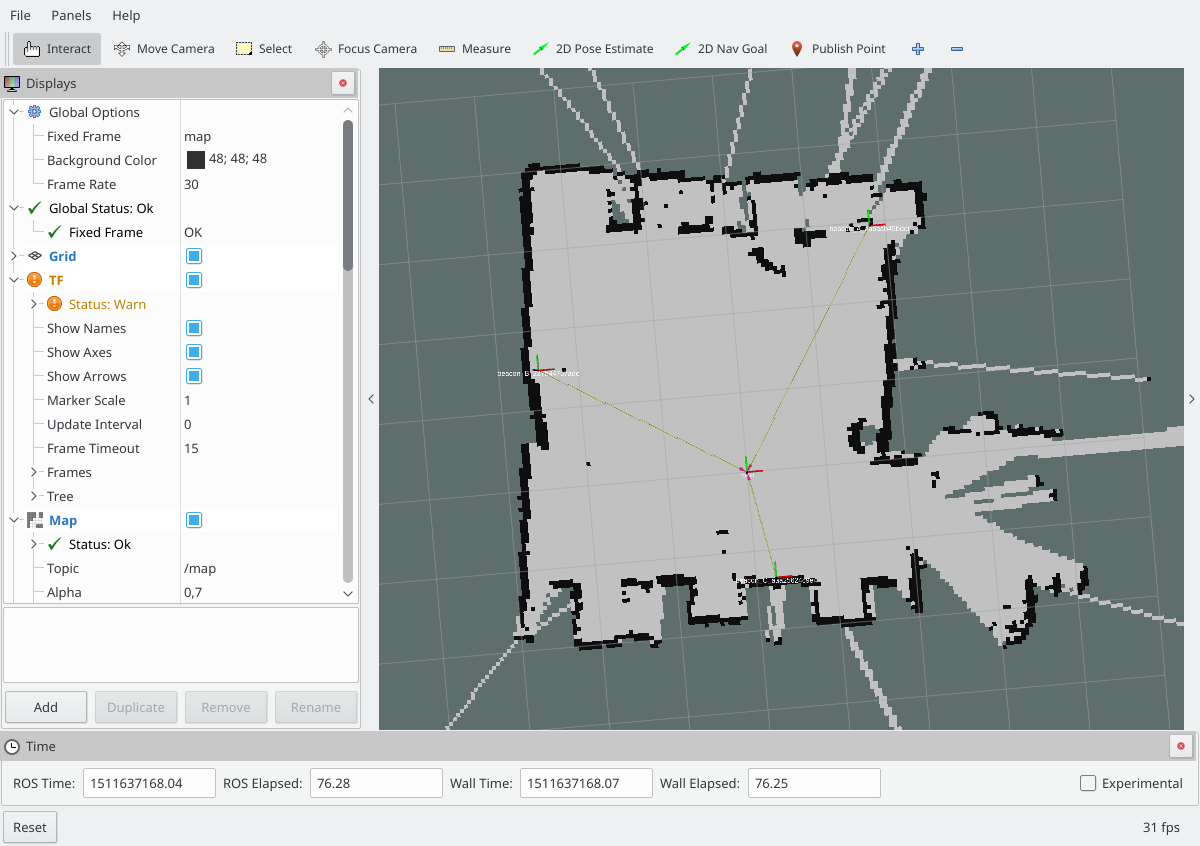
\includegraphics[width=0.8\textwidth]{img/rviz.png}
\caption{Okno programu RViz}
\label{fig:rviz}
\end{figure}

\subsubsection{Gmapping}
Gmapping jest narzędziem należącym do pakietu OpenSLAM, służącym do budowania dwuwymiarowych map pomieszczeń za pomocą SLAM (Simultaneous Localization And Mapping, ang. \textit{Jednoczesna Lokalizacja i Mapowanie}). Program wykorzystuje pomiar ze skanera laserowego oraz odometrię. 

\subsubsection{Rosbag}
Program Rosbag pozwala na zapisywanie do pliku danych publikowanych w wybranych tematach wraz z ich znacznikami czasowymi, celem późniejszego odtworzenia. Narzędzie to pozwoliło na nagranie szeregu testowych przejazdów robota, celem późniejszego zbudowania mapy pomieszczenia i wykonania pomiarów. Zaawansowane funkcjonalności manipulowania zegarem systemu ROS pozwalają na integrowanie danych odtwarzanych za pomocą Rosbag z danymi generowanymi w czasie rzeczywistym.

\subsubsection{Dodatkowe skrypty}
W ramach testów systemu przygotowano także szereg dodatkowych skryptów w języku Python:
\begin{itemize}
 \item skrypt do zbierania danych RSSI do pliku tekstowego, celem dalszej obróbki,
 \item skrypt do dopasowania modelu \ref{eq:logfit_d} do danych pomiarowych.
\end{itemize}


\section{Zmienność wartości siły sygnału RSSI}
\label{sec:zmiennosc}
\subsection{Metodyka badań}
Przedmiotem niniejszego eksperymentu było zbadanie przebiegu wartości RSSI w czasie dla sytuacji, w której nadajnik i odbiornik są nieruchome. Dodatkowo, wyznaczono histogramy wartości RSSI celem aproksymowania dystrybucji prawdopobieństwa wartości RSSI. 

Wykorzystano znacznik opisany w rozdziale \ref{subsec:znacznik} oraz odbiornik Wi-Fi/Bluetooth Intel 7260, zamontowany w laptopie Lenovo Y50 działającego pod kontrolą systemu Linux Mint 18. 

Testy przeprowadzono w pomieszczeniu o wymiarach 1.5 x 20 m (korytarz).Pomieszczenie to charakteryzował wysoki poziom zakłóceń radiowych w paśmie ISM (liczne punkty dostępowe Wi-Fi i odbiorniki elektryczne). Znacznik radiowy i odbiornik znajdowały się na wysokości 70 cm nad podłogą. Przeprowadzono pomiar dla odległości 1 m i 5 m. Pomiar polegał na zebraniu 100 wartości siły sygnału RSSI. Tak zebrane dane obrazowano w postaci wykresu czasowego i histogramu. 

\subsection{Wyniki}

Z wykresów \ref{fig:rssi-1m} i \ref{fig:rssi-5m} widać, że siła sygnału RSSI waha się znacznie nawet dla stanu ustalonego. Amplituda wahań dla odległości 1 m jest średnio rzędu 7 dBm. Dla odległości 5 m jest znacznie większa, rzędu 7 m. Stanowi to poważną przeszkodę dla pomiaru odległości za pomocą RSSI - kumulują się bowiem dwa negatywne czynniki: po pierwsze zależność RSSI od odległości jest w zakresie powyżej 2 m niemal płaska, po drugie - występują duże wahania wartości RSSI, które w tym zakresie będą się przekładać na znaczne wahania odległości. 

Wykresy \ref{fig:rssi-1m-hist} i \ref{fig:rssi-5m-hist} zawierają histogramy wygenerowane z danych pomiarowych. Dla odległości 1 m rozkład wyników pomiarów jest zbliżony do Gaussowskiego, jednak dla 5 m obserwujemy wyraźną asymetrię w kierunku niższych wartości siły sygnału. Jest to wynik wymienionych w rozdziale \ref{ch:radio} zakłóceń, szczególnie wielokrotnych odbić od ścian pomieszczenia. Także szerokość rozkładu jest większa niż w wypadku odległości 1 m. 

\begin{figure}[H]
\centering
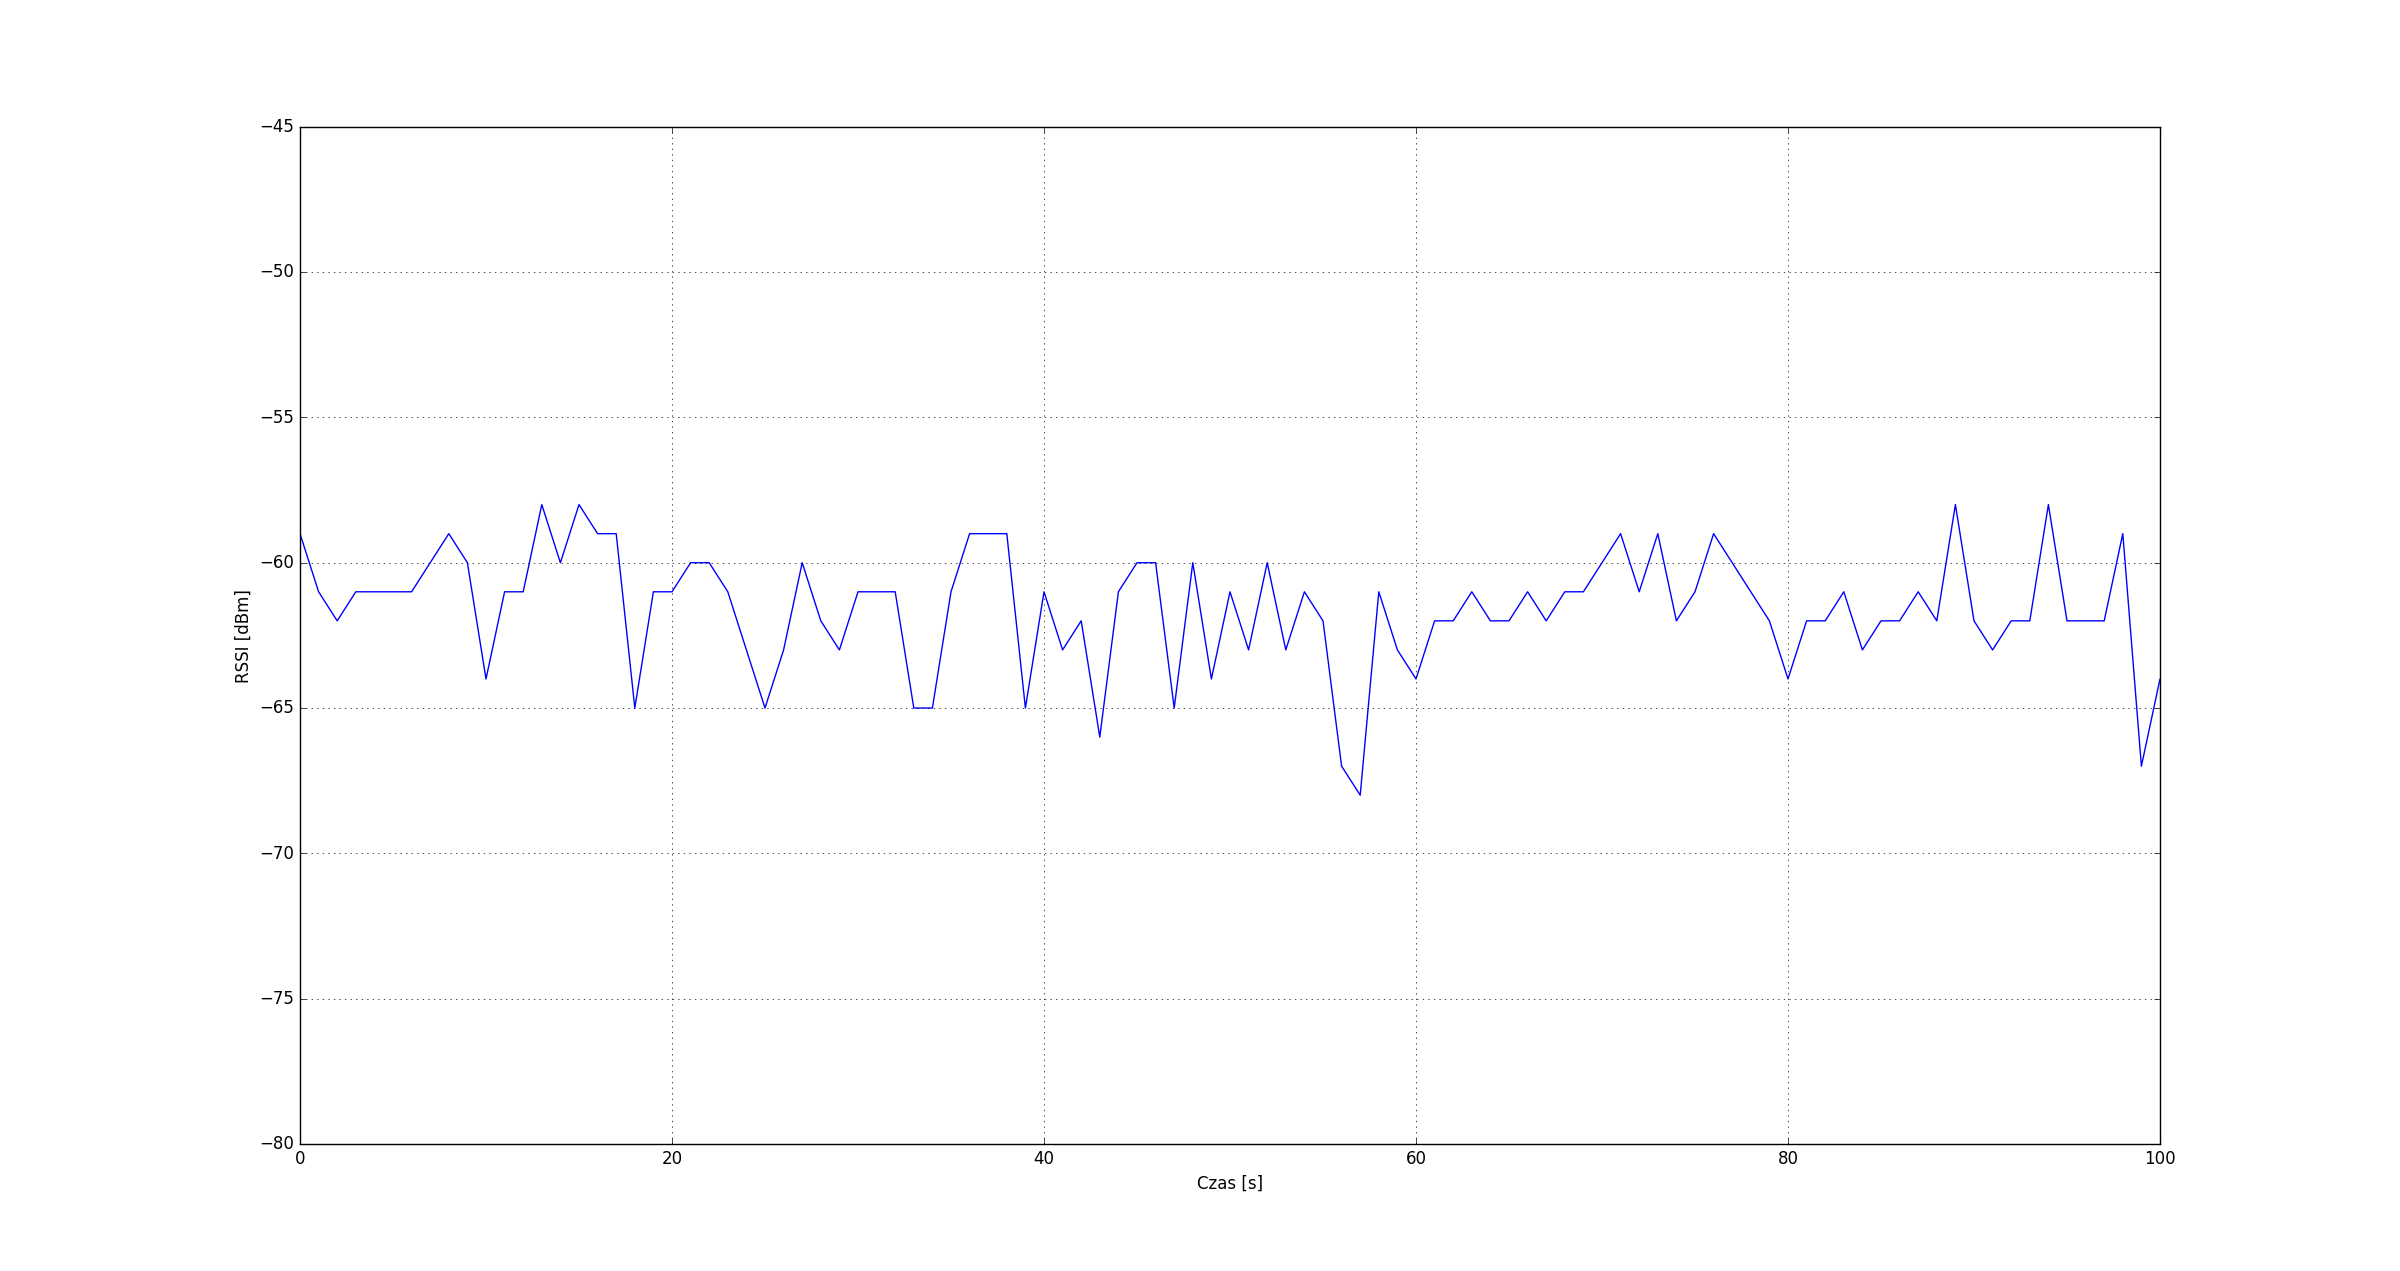
\includegraphics[width=1\textwidth]{img/1m.png}
\caption{Przebieg wartości siły sygnału RSSI w czasie dla odległości odbiornika od nadajnika równej 1 m}
\label{fig:rssi-1m}
\end{figure}

\begin{figure}[H]
\centering
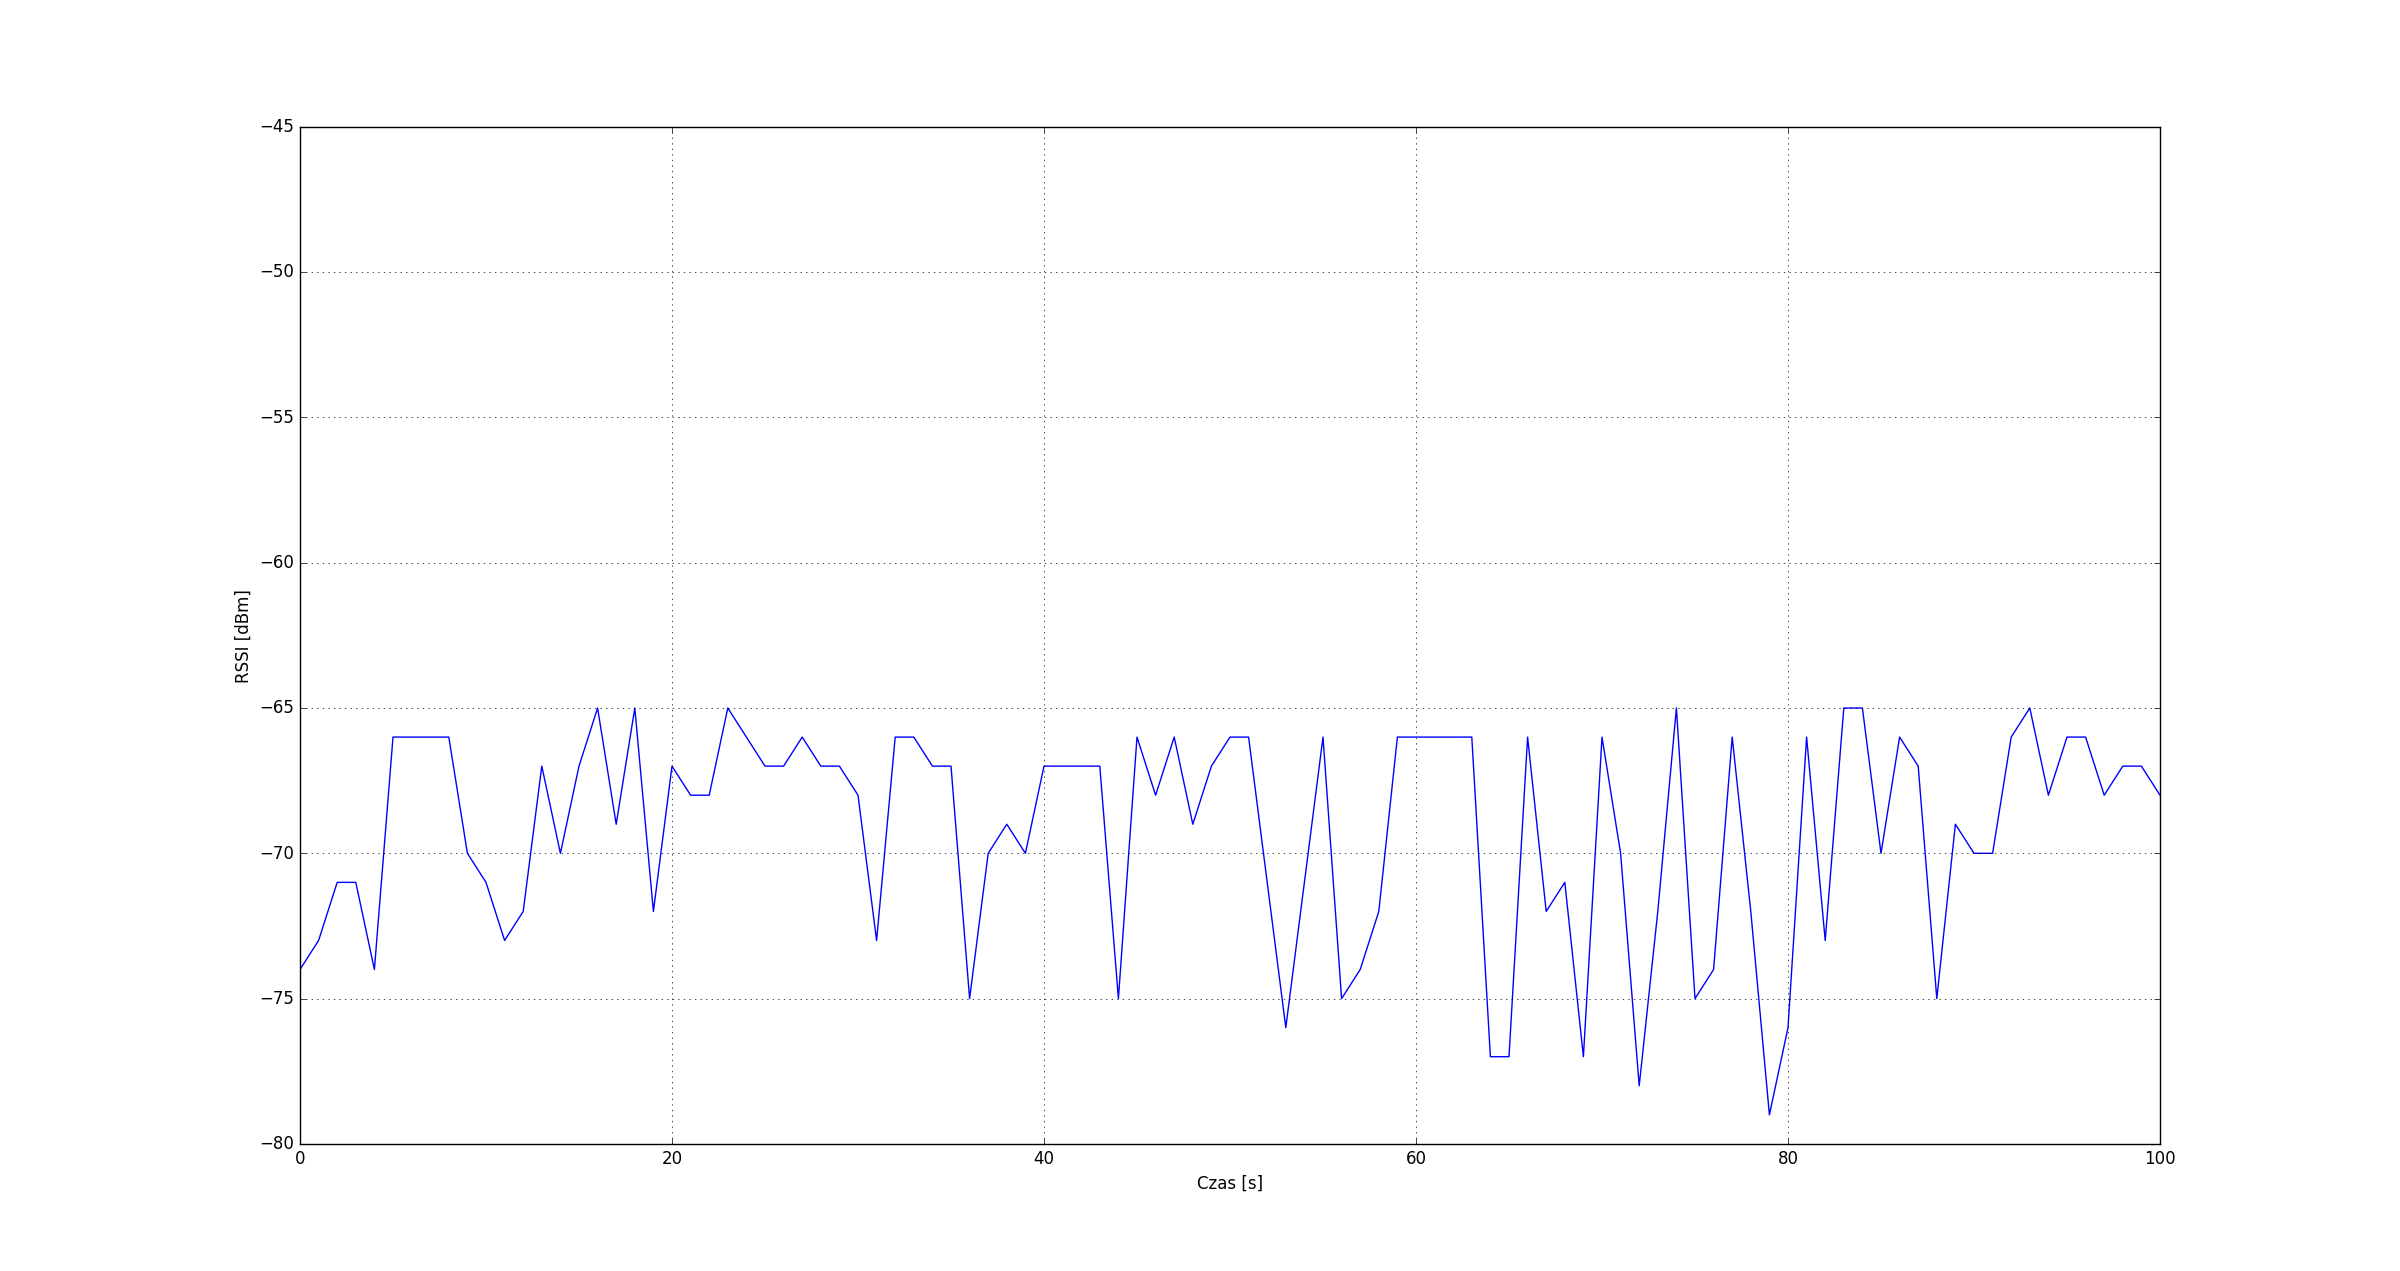
\includegraphics[width=1\textwidth]{img/5m.png}
\caption{Przebieg wartości siły sygnału RSSI w czasie dla odległości odbiornika od nadajnika równej 1 m}
\label{fig:rssi-5m}
\end{figure}

\begin{figure}[H]
\centering
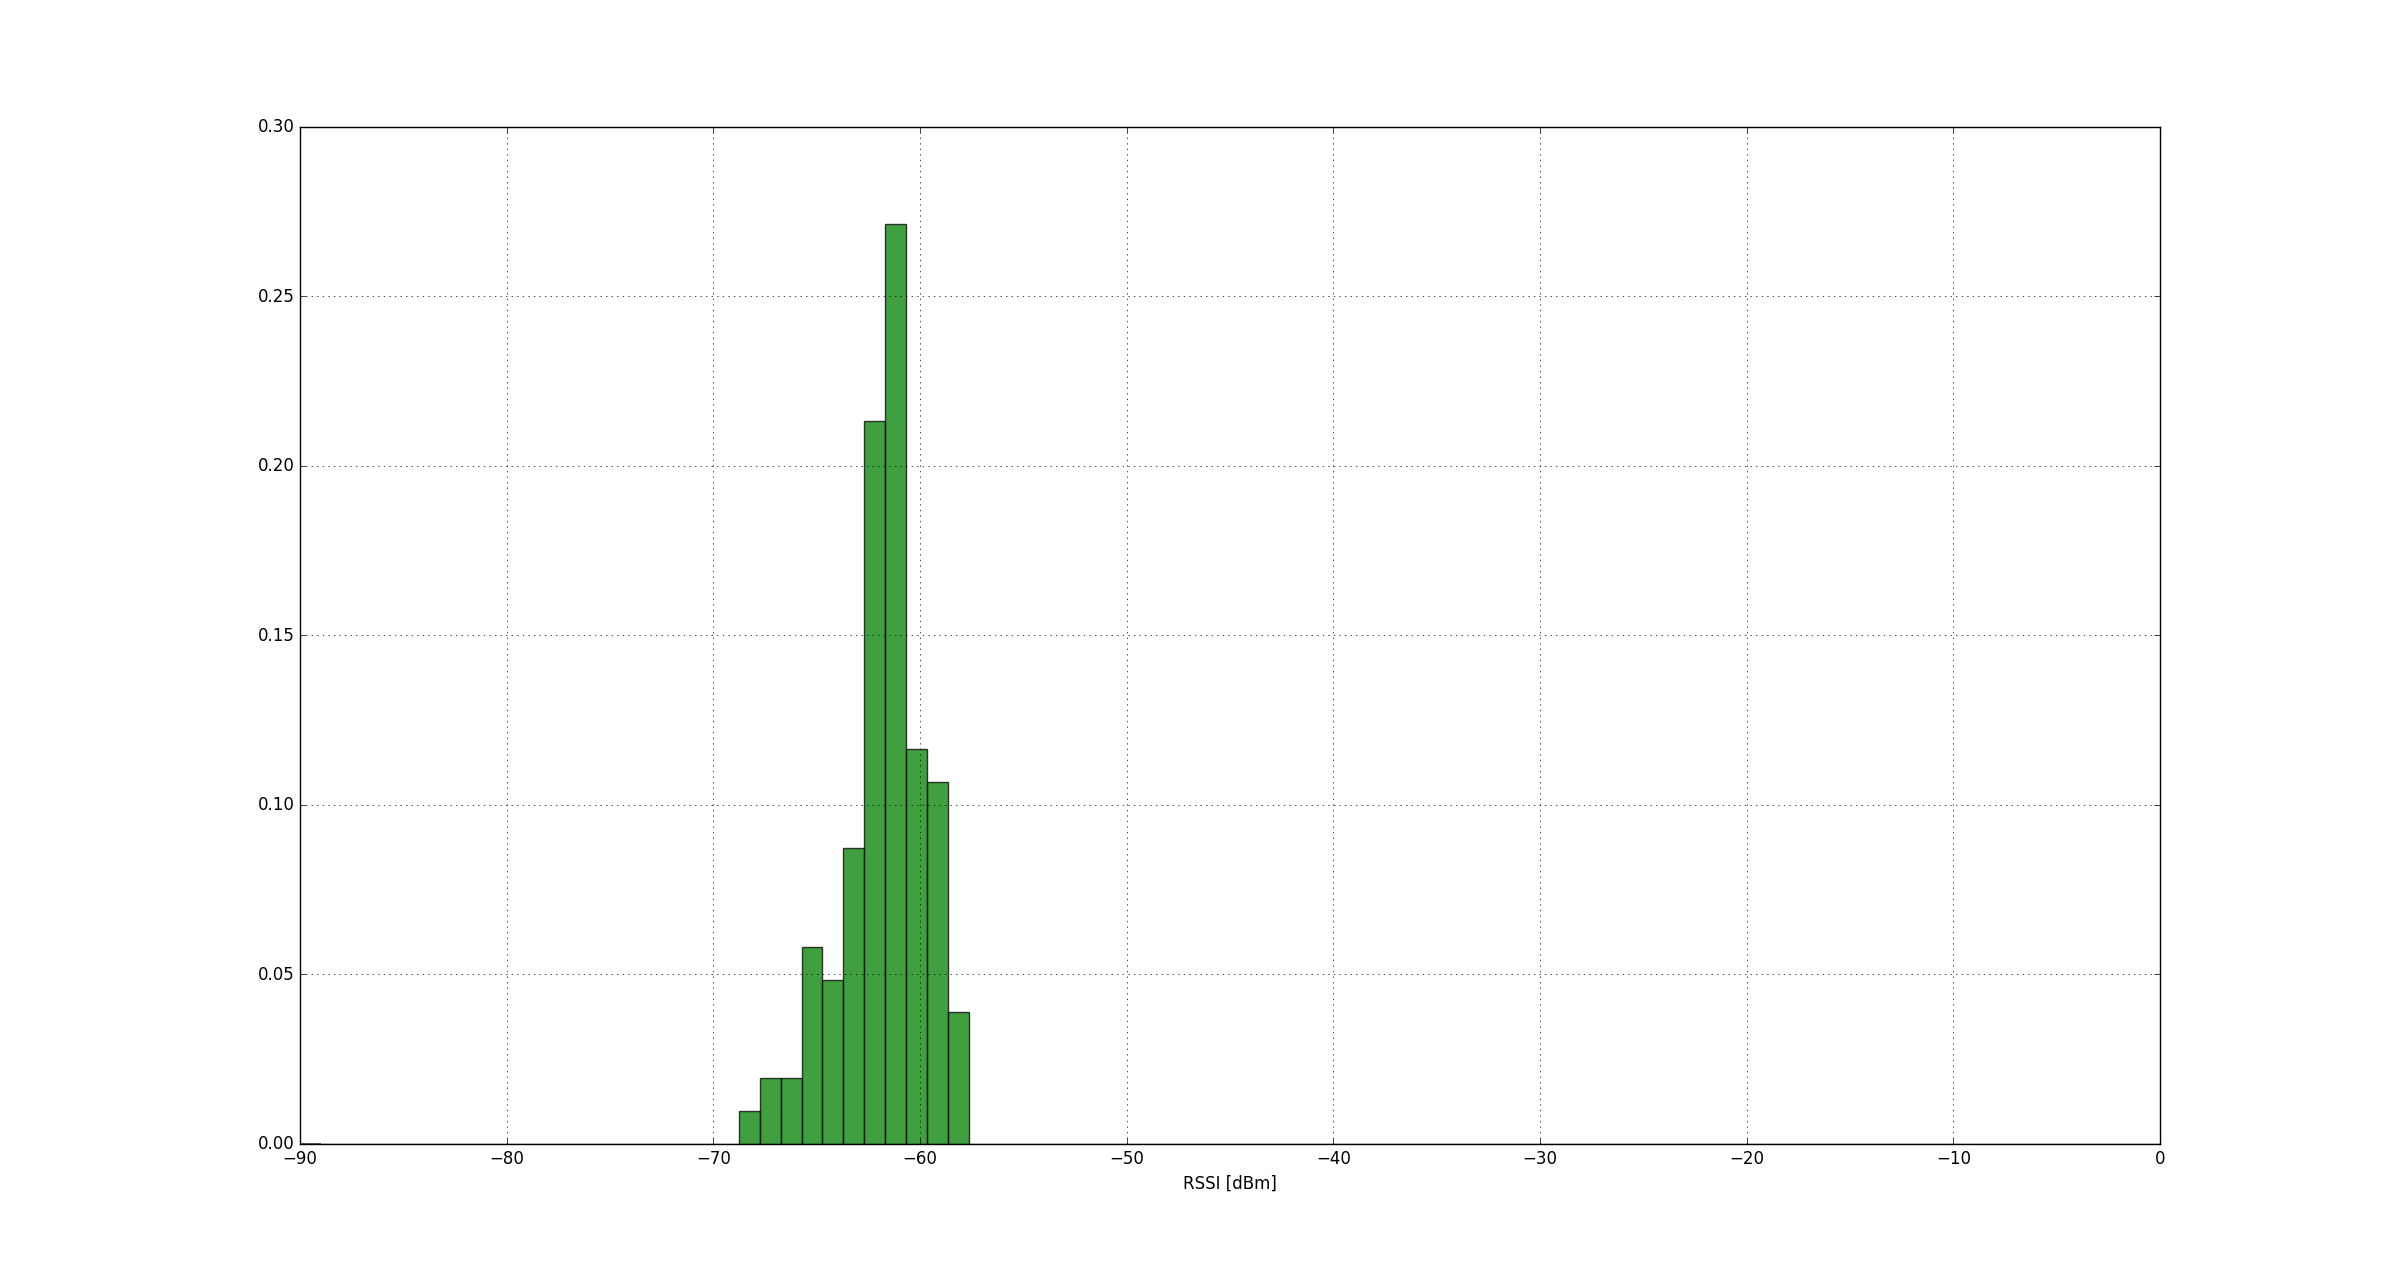
\includegraphics[width=1\textwidth]{img/1m-hist.png}
\caption{Histogram siły sygnału RSSI w czasie dla odległości odbiornika od nadajnika równej 1 m}
\label{fig:rssi-1m-hist}
\end{figure}

\begin{figure}[H]
\centering
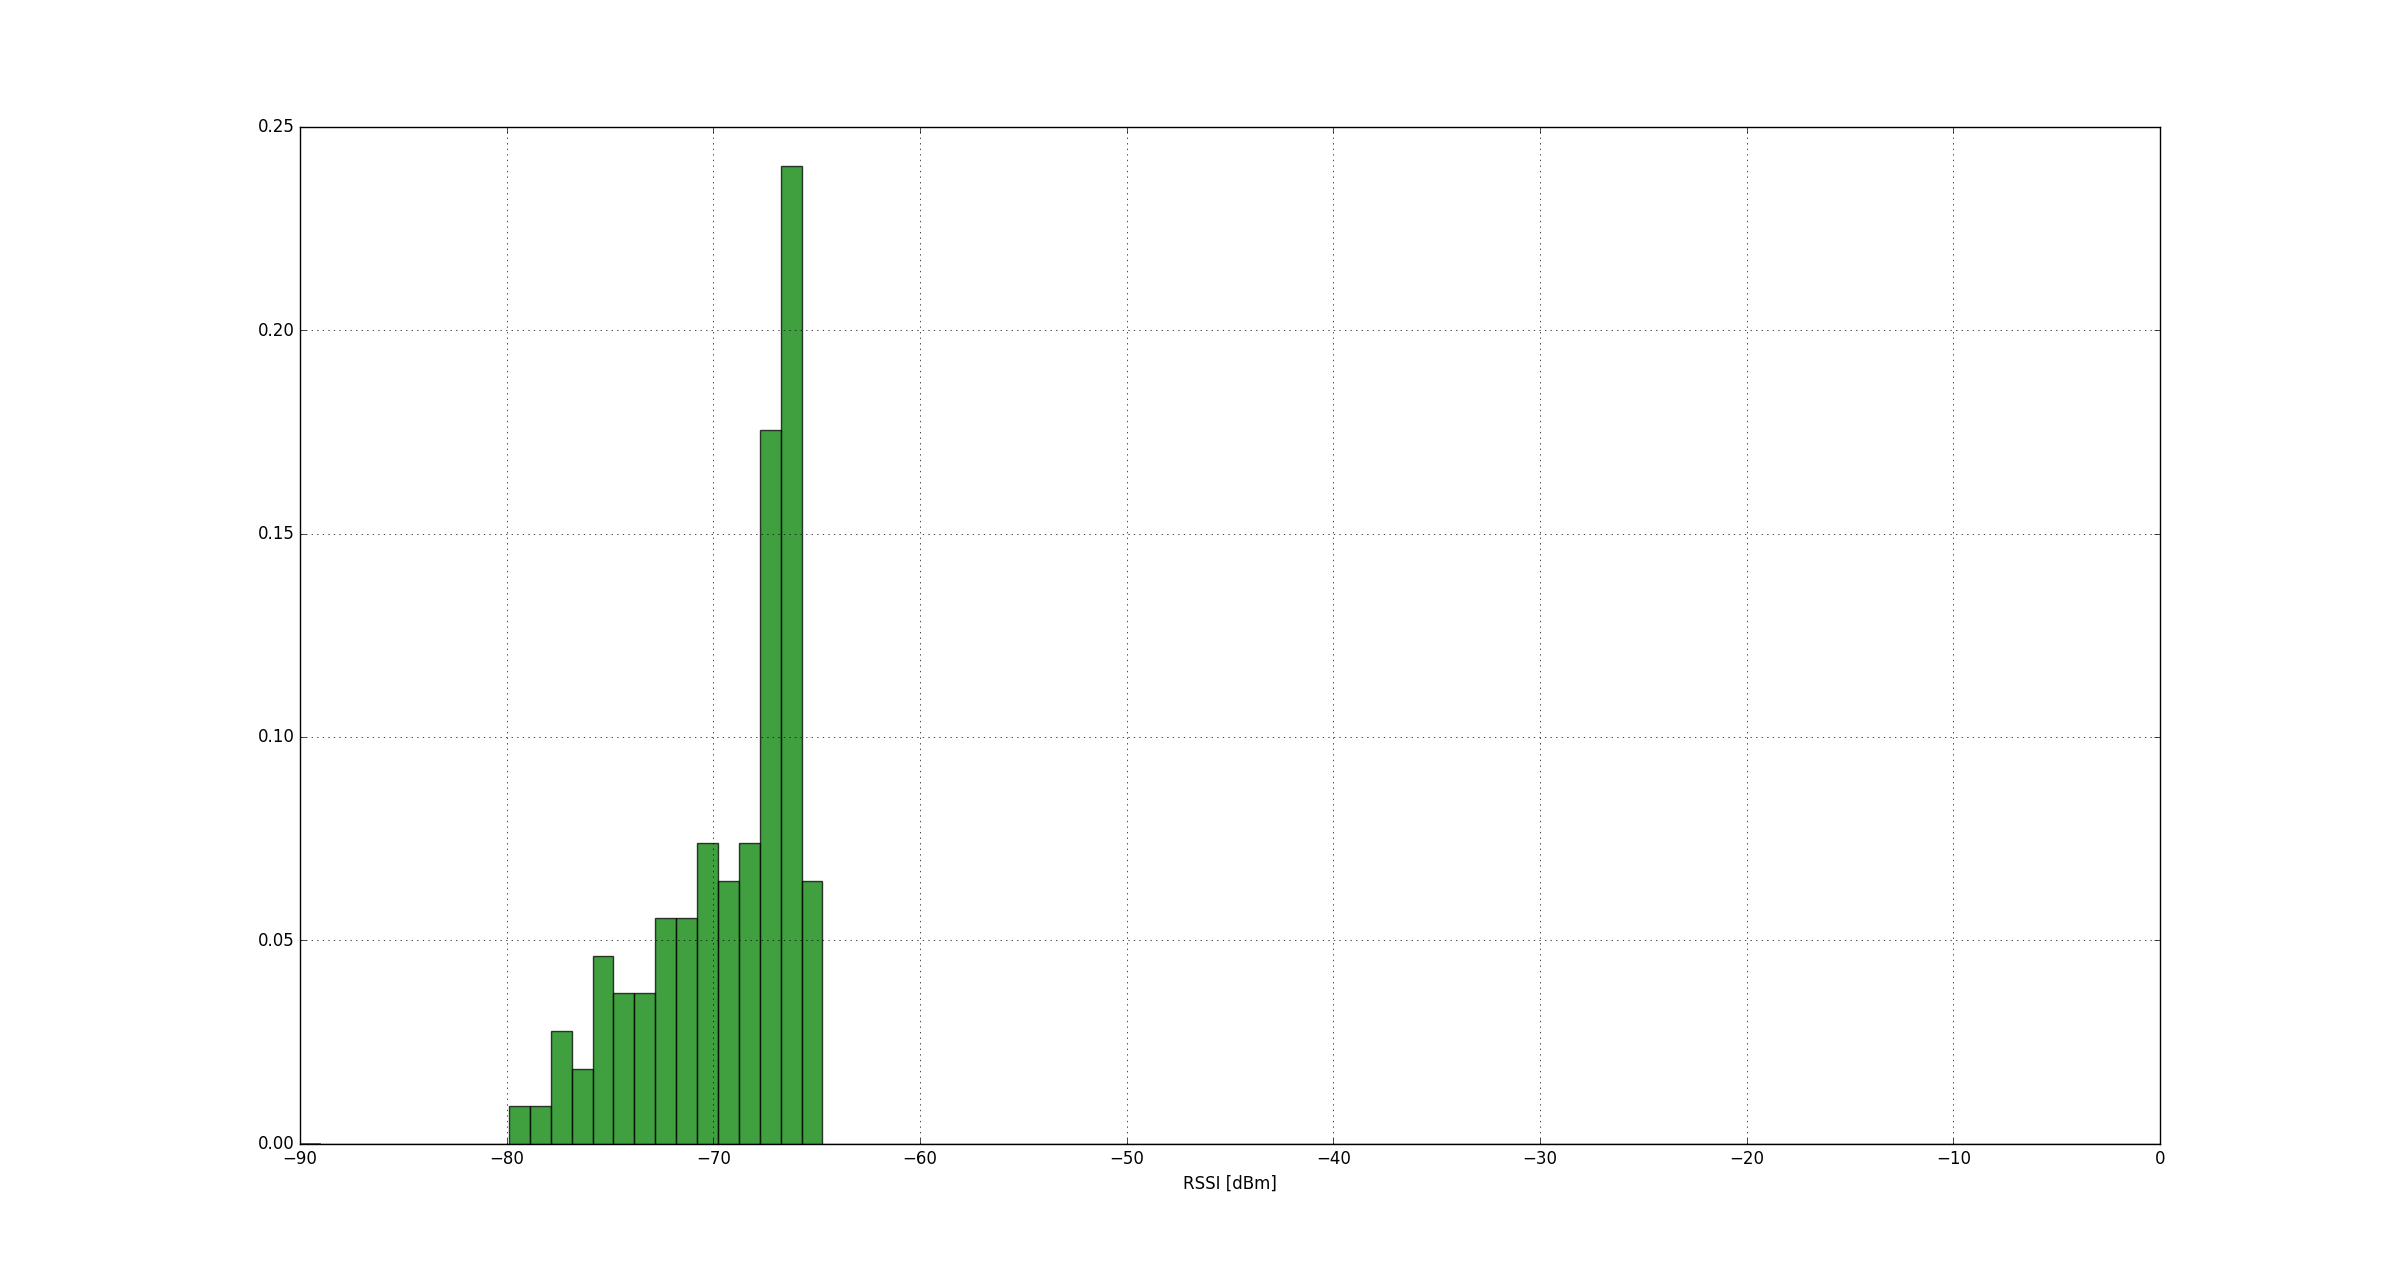
\includegraphics[width=1\textwidth]{img/5m-hist.png}
\caption{Histogram siły sygnału RSSI w czasie dla odległości odbiornika od nadajnika równej 1 m}
\label{fig:rssi-5m-hist}
\end{figure}


\section{Zależność siły sygnału RSSI od odległości}

\subsection{Metodyka badań}
Celem niniejszego eksperymentu jest zweryfikowanie modelu przedstawionego w rozdziale \ref{ch:radio}. Środowisko testowe było identyczne jak w punkcie \ref{sec:zmiennosc}. W każdym punkcie pomiarowym zebrano 30 próbek RSSI, które następnie uśredniono i wyznaczono odchylenie standardowe. Następnie wykonano dopasowanie krzywych logarytmicznych według metody interpolacji oraz dopasowania krzywej (por. rozdział \ref{sec:rssi-odleglosc}).

\subsection{Wyniki}

Na wykresie \ref{fig:odleglosc-rssi} widać logarytmiczną zależność pomiędzy odległością, a wartością siły sygnału RSSI, zgodną z oczekiwaniami teoretycznymi opisanymi w \ref{eq:model_propag}. Jednocześnie wraz ze wzrostem odległości od nadajnika, wzrasta odchylenie standardowe pomiarów, co oznacza że wahania wartości RSSI były większe. 

W odległości 3.5m oraz 5 m obserwujemy niewielki wzrost siły sygnału RSSI, co może wskazywać, że w tych miejscach środowiska testowego zachodziły warunki powodujące lokalne wzmocnienie fali. 
Należy zwrócić uwagę, iż w zakresie odległości powyżej 2 m wartość RSSI pozostaje na stałym poziomie, wahając się w granicach 10 dBm. Z tego powodu jakość pomiaru odległości za pomocą RSSI w tym zakresie będzie bardzo słaba. 

Wykres \ref{fig:odleglosc-rssi-fit} ukazuje dopasowane do wyników pomiaru krzywe: metodą interpolacji (\ref{eq:interpol}) i poprzez dopasowanie krzywej \ref{eq:logfit_d} za pomocą funkcji \textit{curve{\_}fit} z bilbioteki \textit{scipy} dla języka Python. Należy zwrócić uwage, iż w porównaniu z wykresem \ref{fig:odleglosc-rssi} zamienione zostały osie układu współrzędnych, tj. wykres \ref{fig:odleglosc-rssi-fit} przedstawia problem z perspektywy przeliczania RSSI na odleglość. 

Funkcja \textit{curve{\_}fit} uwzględnia wszystkie punkty pomiarowe wraz z ich niepewnościami, dlatego zapewnia lepsze dopasowanie od interpolacji, biorącej pod uwagę tylko dwa punkty pomiarowe. Jednakże, aby osiągnąć zadowalające dopasowanie, trzeba albo ręcznie wybrać dwa optymalne punkty do dopasowania interpolacyjnego, albo usunąć punkty zbyt odstające od pozostałych dla metody dopasowania krzywej. 

\begin{figure}[ht]
\centering
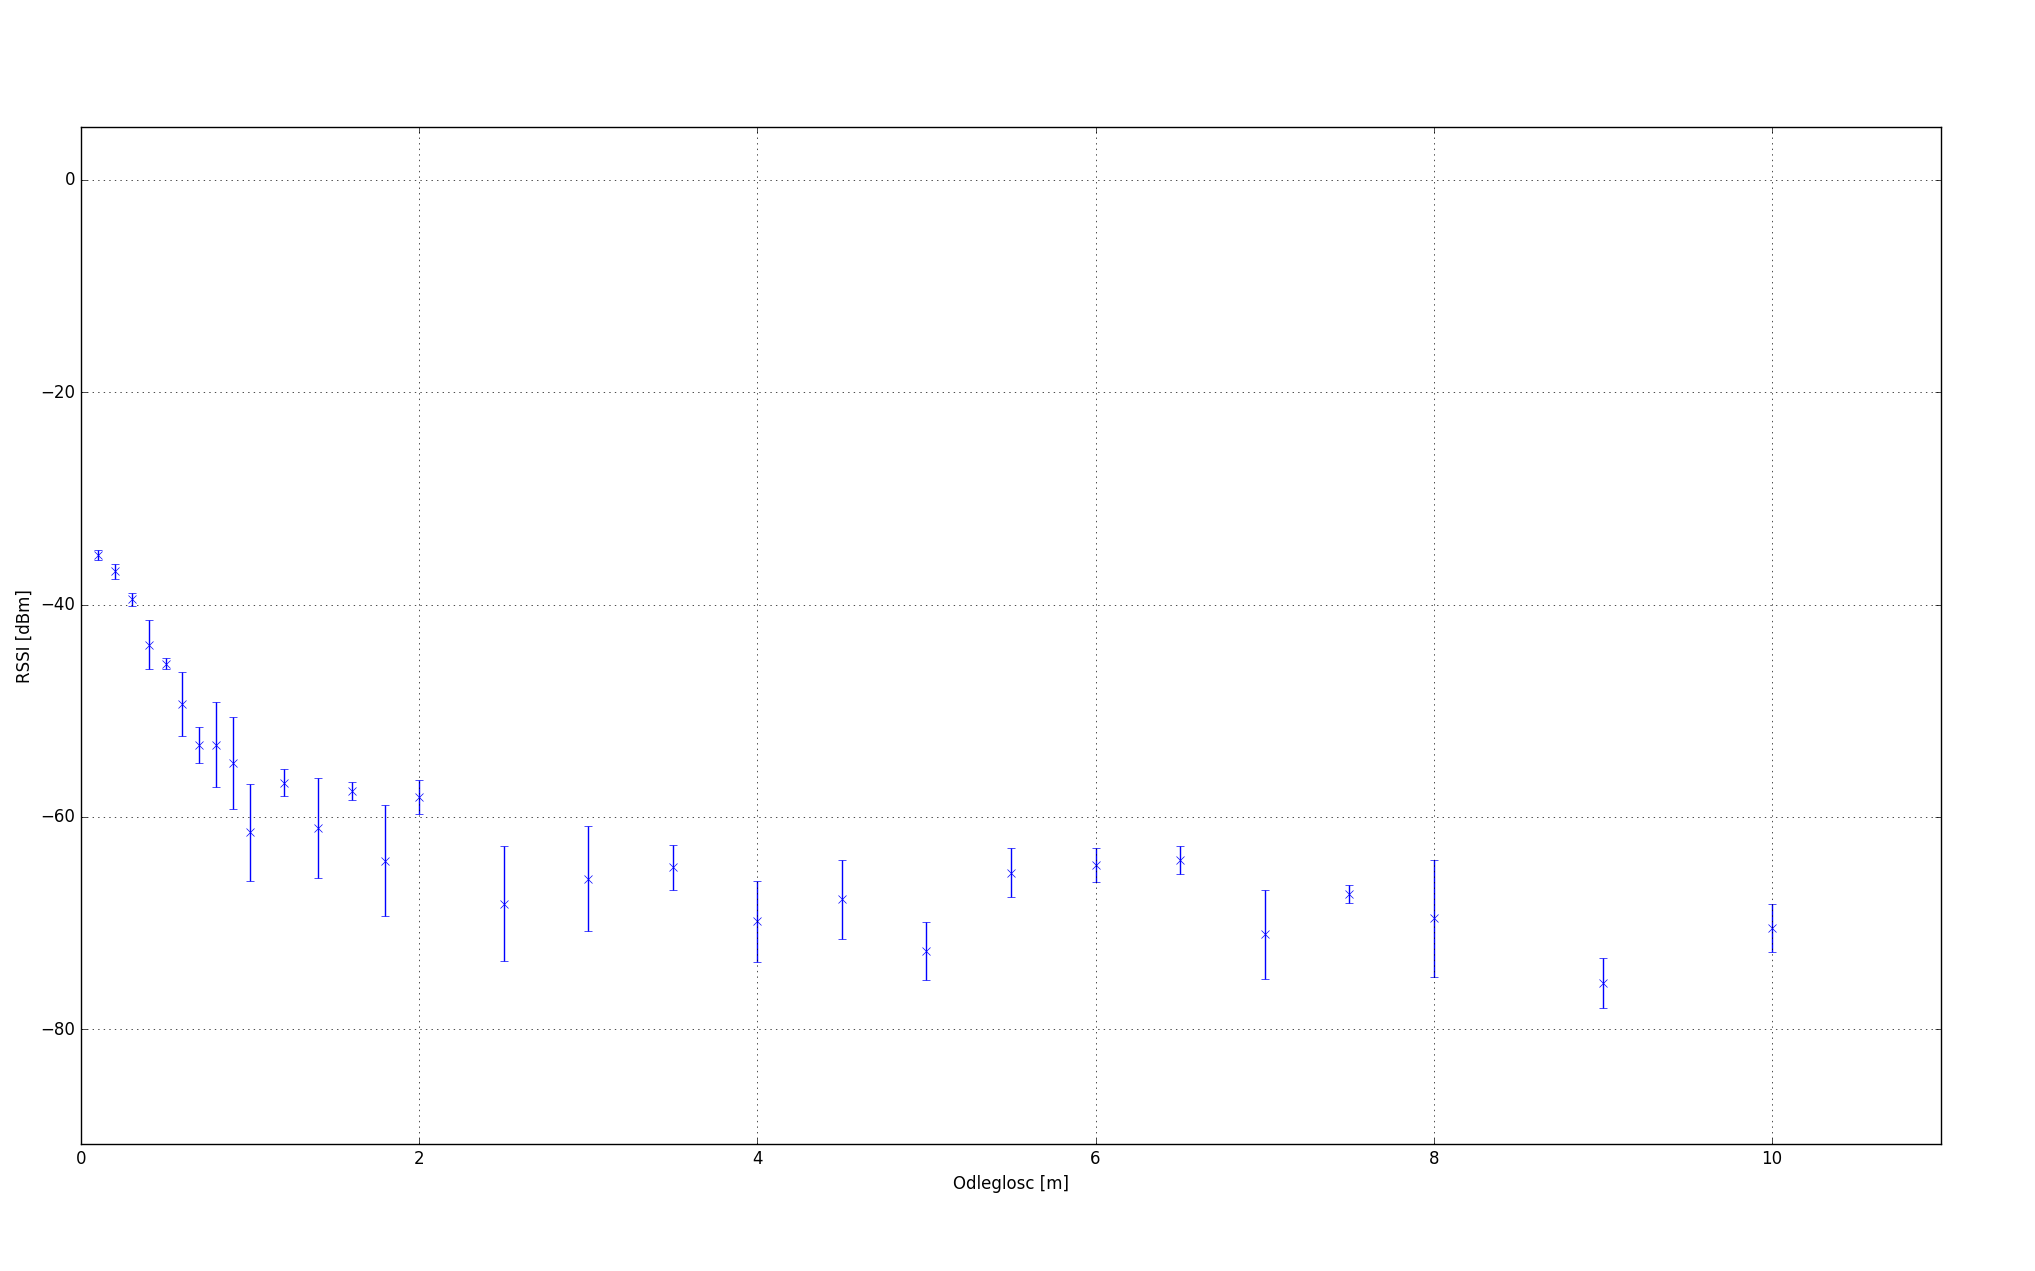
\includegraphics[width=1\textwidth]{img/odleglosc-rssi.png}
\caption{Wykres wartości siły sygnału RSSI w zależności odległości}
\label{fig:odleglosc-rssi}
\end{figure}


\begin{figure}[ht]
\centering
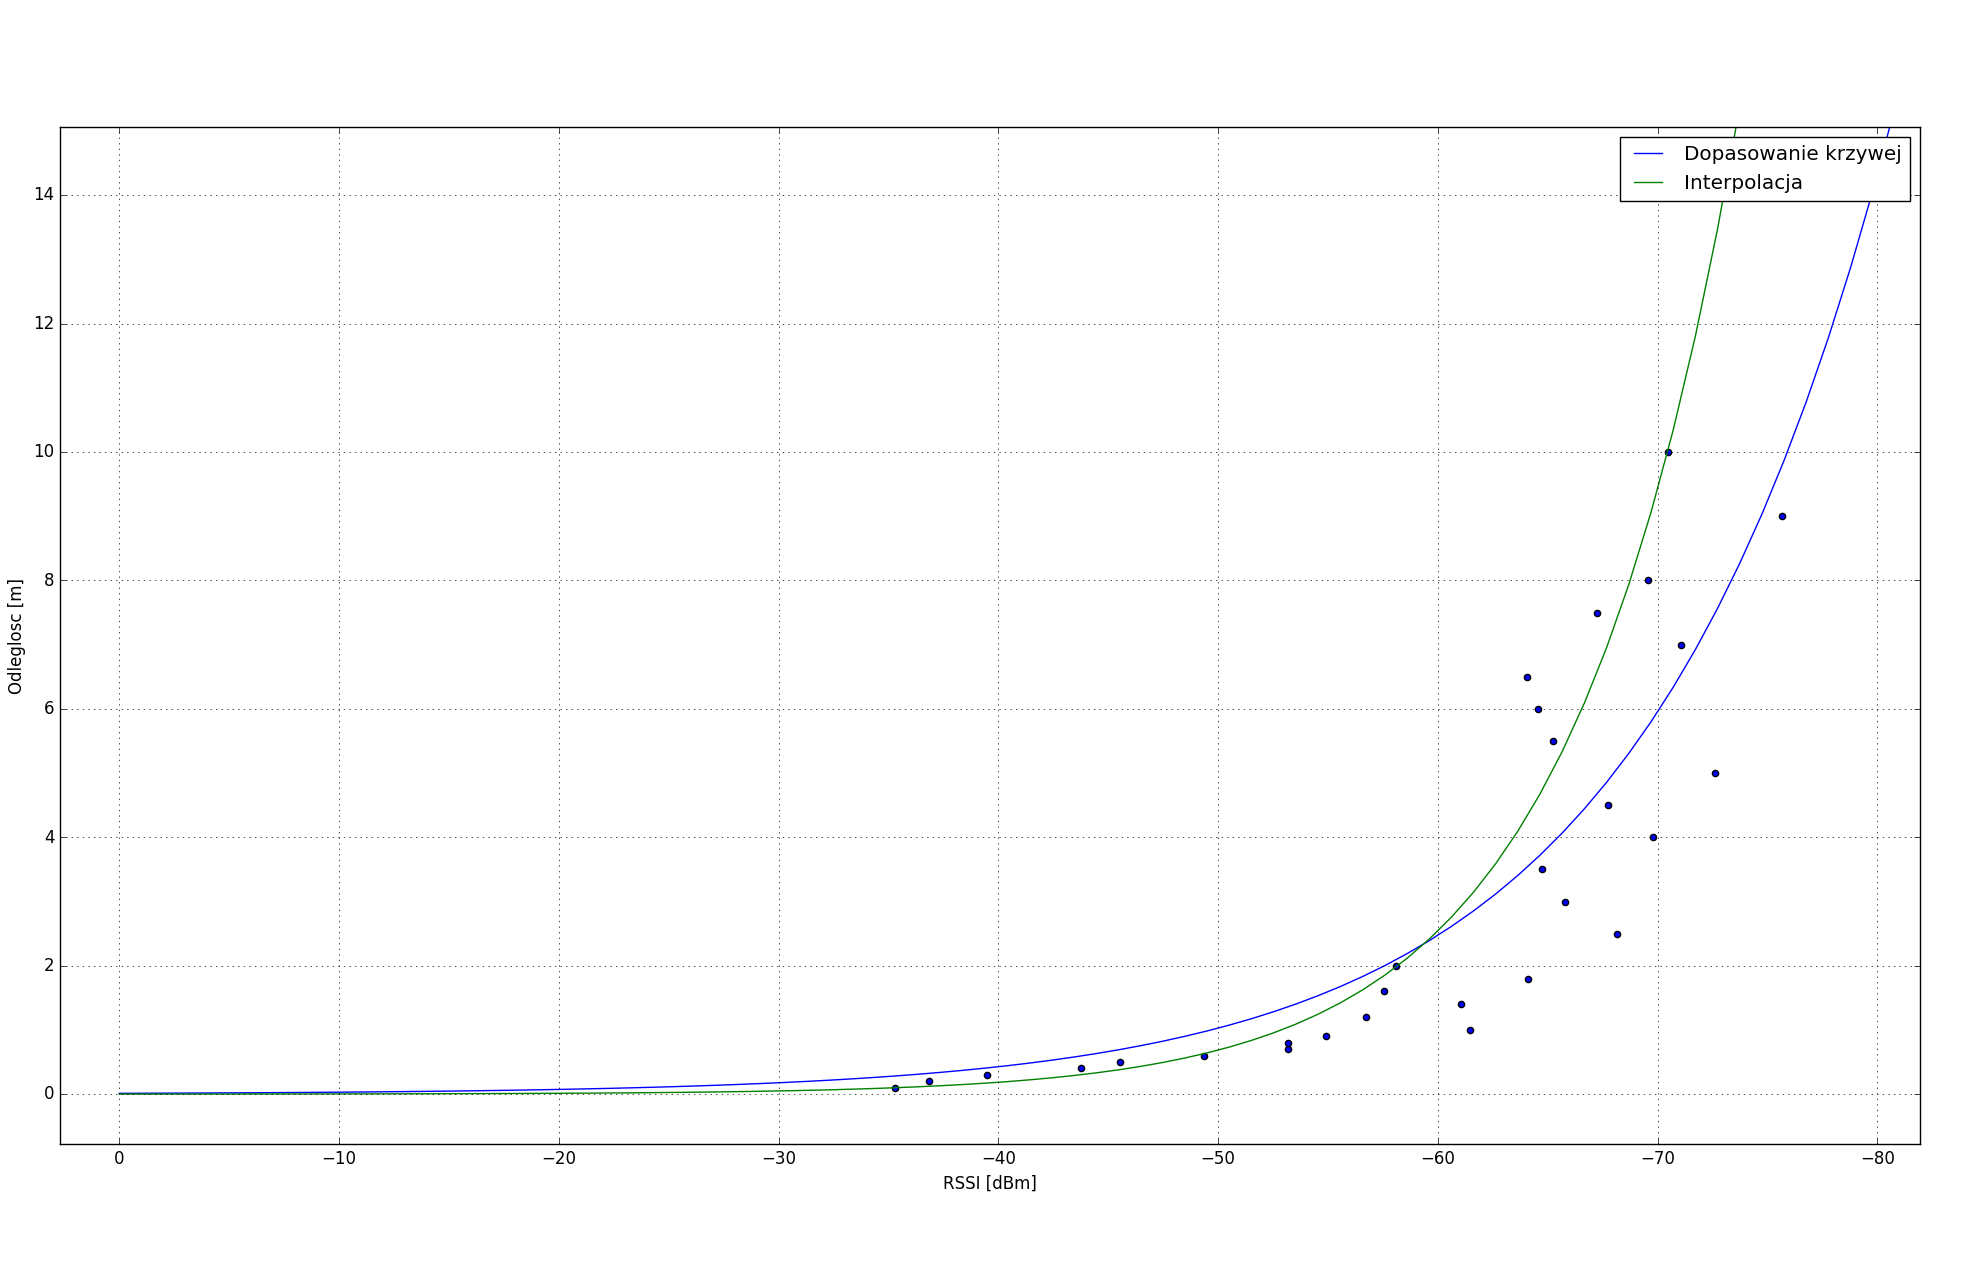
\includegraphics[width=1\textwidth]{img/rssi-odleglosc.png}
\caption{Wykres dopasowania krzywych potęgowych do wyników pomiaru}
\label{fig:odleglosc-rssi-fit}
\end{figure}

\section{Porównanie metod filtracji siły sygnału RSSI}
\label{sec:testy-filtracja}
\subsection{Metodyka badań}
Eksperyment miał na celu porównanie skuteczności metod filtracji sygnału RSSI opisanych w \ref{sec:rssi-odleglosc}. Pożądanym wynikiem jest dobre wygładzenie stacjonarnych wahań RSSI przy zachowaniu małej bezwładności, tj. szybkiej reakcji na rzeczywistą zmianę siły sygnału RSSI, wynikłą ze zmiany odległości od znacznika. 

W ramach eksperymentu posłużono się zbiorem danych nagranym za pomocą programu rosbag. Obejmował on pomiary RSSI zbierane z interwałem 1 sekundy, dla następującej sekwencji: przez 40 sekund znacznik pozostaje w odległości 1 m od odbiornika, następnie zostaje przeniesiony na odległość 2 m, po kolejnych 20 sekundach zostaje przeniesiony z powrotem na odległość 1 m gdzie pozostaje przez 40 sekund. 

\subsection{Wyniki}
Filtr średniej ruchomej (por. \ref{subsec:filtracja_rssi}) wprowadza znaczną bezwładność do układu (por. rys \ref{fig:filtry-avg}), przy czym dla większej liczby kroków średniej $N = 10$ bezwładność nie jest znacząco większa. Filtr zapewnia dobre wygładzenie dla nieruchomego odbiornika. W wypadku zmiany odgległości, filtr potrzebuje 10 sekund aby dość do stanu ustalonego, co dyskwalifikuje jego zastosowanie w lokalizacji dynamicznej. 

\begin{figure}[ht]
\centering
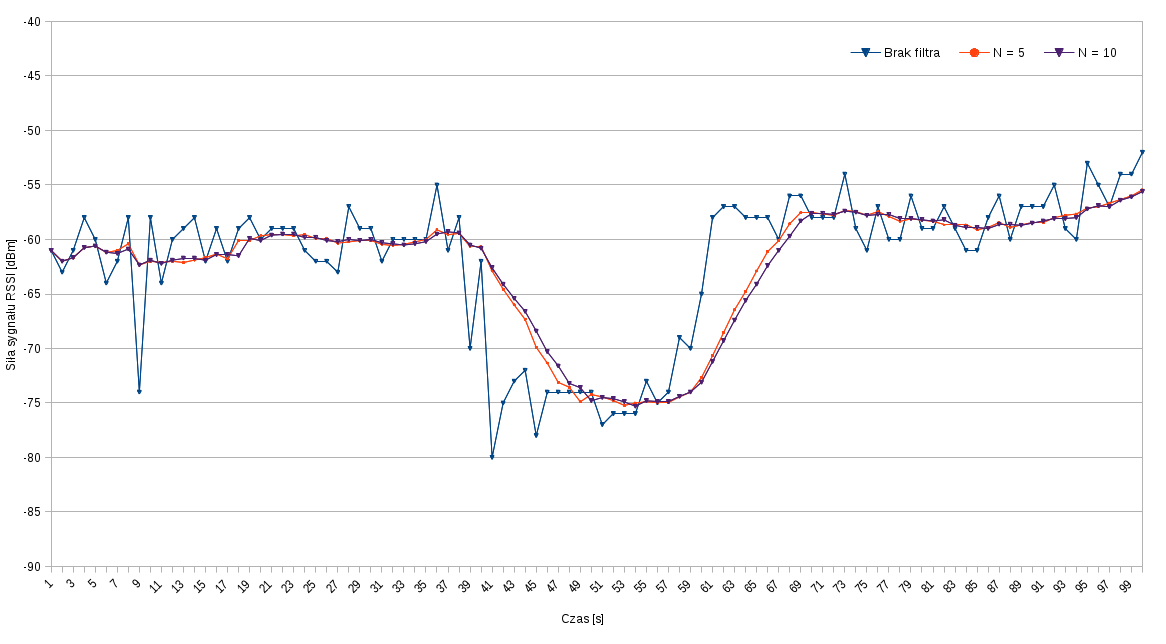
\includegraphics[width=0.9\textwidth]{img/filtr-avb.png}
\caption{Filtr średniej ruchomej}
\label{fig:filtry-avg}
\end{figure}

Filtr probablistyczny jest strojony za pomocą dwóch parametrów: $a$ - opisujący jak istotna jest wartość poprzedniego pomiaru w estymacji bieżącego, oraz $b$ - opisujący jak istotny jest przyrost wartości RSSI. Innymi słowy, parametr $a$ opisuje wygładzanie filtra, zaś $b$ opisuje czułość na zmiany RSSI. Zbyt niska wartość $a$ powoduje dużą bezwładność filtra, z kolei wartość $a=1$ powoduje że wartość estymowana jest wartości zmierzonej. Zbyt duża wartość $b$ spowoduje oscylacje, a nawet utratę stabilności filtra. 

W eksperymencie porównano dwa zestawy nastaw filtra (rys. \ref{fig:filtry-probab}):
\begin{itemize}
 \item \textbf{Nastawy 1} $a=0.35$ $b=0.02$
 \item \textbf{Nastawy 2} $a=0.15$ $b=0.005$
\end{itemize}

Nastawy 2 zapewniają dobre wygładzenie w stanie ustalonym oraz bardzo dużą bezwładność. Zwiększanie parametru $b$ spowoduje jedynie zaistnienie oscylacji, bez poprawy reakcji filtra. 

Z kolei nastawy 1 stanowią dobry kompromis pomiędzy wygładzeniem a reakcją na zmiany RSSI. Filtr reaguje na zmianę odległości w ciągu około 4 sekund, zaś amplituda wahań wartości w stanie ustalonym jest rzędu 3 dBm. 
\begin{figure}[ht]
\centering
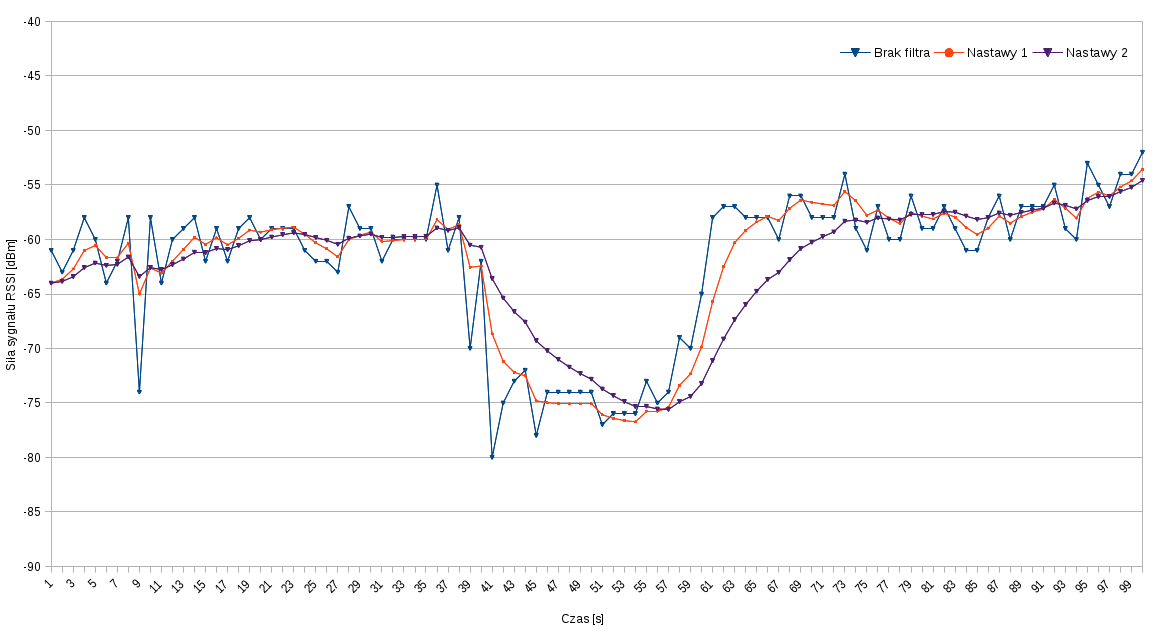
\includegraphics[width=0.9\textwidth]{img/filtr-propab.png}
\caption{Filtr probabilistyczny}
\label{fig:filtry-probab}
\end{figure}
Na wykresie \ref{fig:filtry-wszystkie} przedstawiono przebieg RSSI bez filtracji, z filtracją średnią ruchomą dla $N=5$ oraz filtracją probabilistyczną wg. nastaw 1. Filtr średniej ruchomej ma znacznie większą bezwładność od filtra probabilistycznego. Dlatego do testowania lokalizacji robota wykorzystano właśnie filtr probabilistyczny, jako lepiej radzący sobie w sytuacjach dynamiczych. 
\begin{figure}[H]
\centering
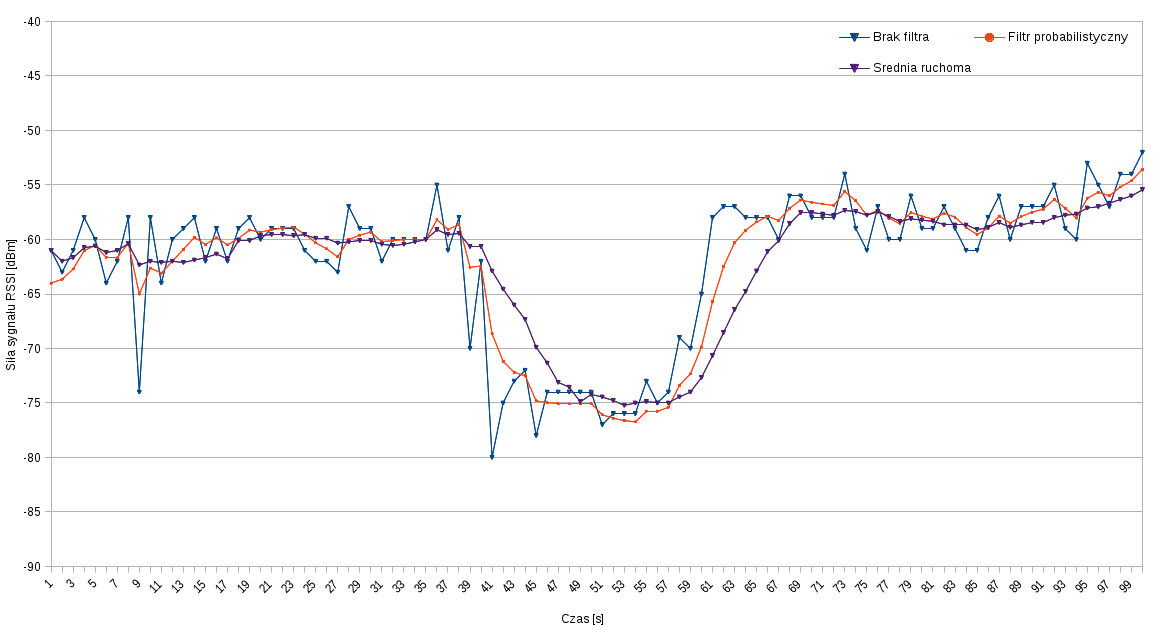
\includegraphics[width=0.9\textwidth]{img/filtry-porownanie.png}
\caption{Porównanie metod filtracji}
\label{fig:filtry-wszystkie}
\end{figure}

\section{Porównanie metod lokalizacji}
W niniejszej sekcji opisano przebieg i wyniki badania zasadniczej części niniejszej pracy - algorytmu lokalizacji. W celu wykonania badań, konieczne było zbudowanie mapy środowiska pracy robota oraz skalibrowanie znaczników, tj. wyznaczenie parametrów modelu \ref{eq:logfit_d}. 
\subsection{Metodyka badań}
Badania metod lokalizacji przeprowadzono na opisanym w rozdziale \ref{sec:hardware} robocie Pioneer 3-AT, w pomieszczeniu Laboratorium Robotyki Mobilnej Wydziału Mechatroniki PW. Do zbudowania mapy pomieszczenia, potrzebnej do pomiarów, wykorzystano program Gmapping. Budowanie mapy polegało na wykonaniu 3 przejazdów dookoła pomieszczenia. W trakcie przejazdów unikano gwałtownych przyspieszeń, hamowań i skrętów robota, w celu ograniczenia uślizgu kół, który wprowadza błąd do mapowania SLAM. 
Tak wyznaczoną mapę zapisano w pliku graficznym PNG. Jeden piksel obrazka reprezentował 5 cm przestrzeni. Następnie zlokalizowano na mapie umiejscowienie znaczników, korzystając z punktów charakterystycznych. 

W celu skalibrowania znaczników zebrano szereg punktów pomiarowych w różnych odległościach od znacznika. Aby wyeliminować wpływ wahań RSSI na wyznaczony model, każdy pomiar składał się z 20 uśrednionionych wartości RSSI.  Następnie wyznaczono model w oparciu o interpolację i dopasowanie funkcji wykładniczej. 

Do badania metod lokalizacji jako odniesienie wykorzystano lokalizację AMCL. Po wykonaniu kilku przejazdów robota po pomieszczeniu oparta o filtr cząsteczkowy lokalizacja AMCL zapewnia dokładność zbliżoną do rozdzielczości mapy, co najmniej o rząd wielkości lepszą niż dokładność lokalizacji w oparciu o znaczniki. Aby zapewnić rzetelne porównanie metod lokalizacji, posłużono się danymi nagranymi programem Rosbag, zatem obydwie metody zostały użyte na identycznych danych testowych. 

W obydwu metodach porównano wyniki lokalizacji obliczone z odległości przefiltrowanych przez poszczególne filtry (por. \ref{sec:testy-filtracja}).
\subsection{Wyniki}

\subsubsection{Mapa środowiska}
Rysunek \ref{fig:mapa} przedstawia wyznaczoną metodą SLAM mapę laboratorium. Punkty w kolorze szarym oznaczają obszar wolny, zaś w kolorze czarnym - zajęty. Pojedyncze czarne punkty i szare linie stanowią wynik zakłóceń SLAM i nie mają negatywnego wpływu na lokalizację. Obszar w prawym dolnym rogu mapy obrazuje otwarte drzwi do sąsiedniego pomieszczenia, które nie było objęte mapowaniem. Na mapie zobrazowane są pozycje początków układów współrzędnych: mapy oraz 3 znaczników. 
\begin{figure}[H]
\centering
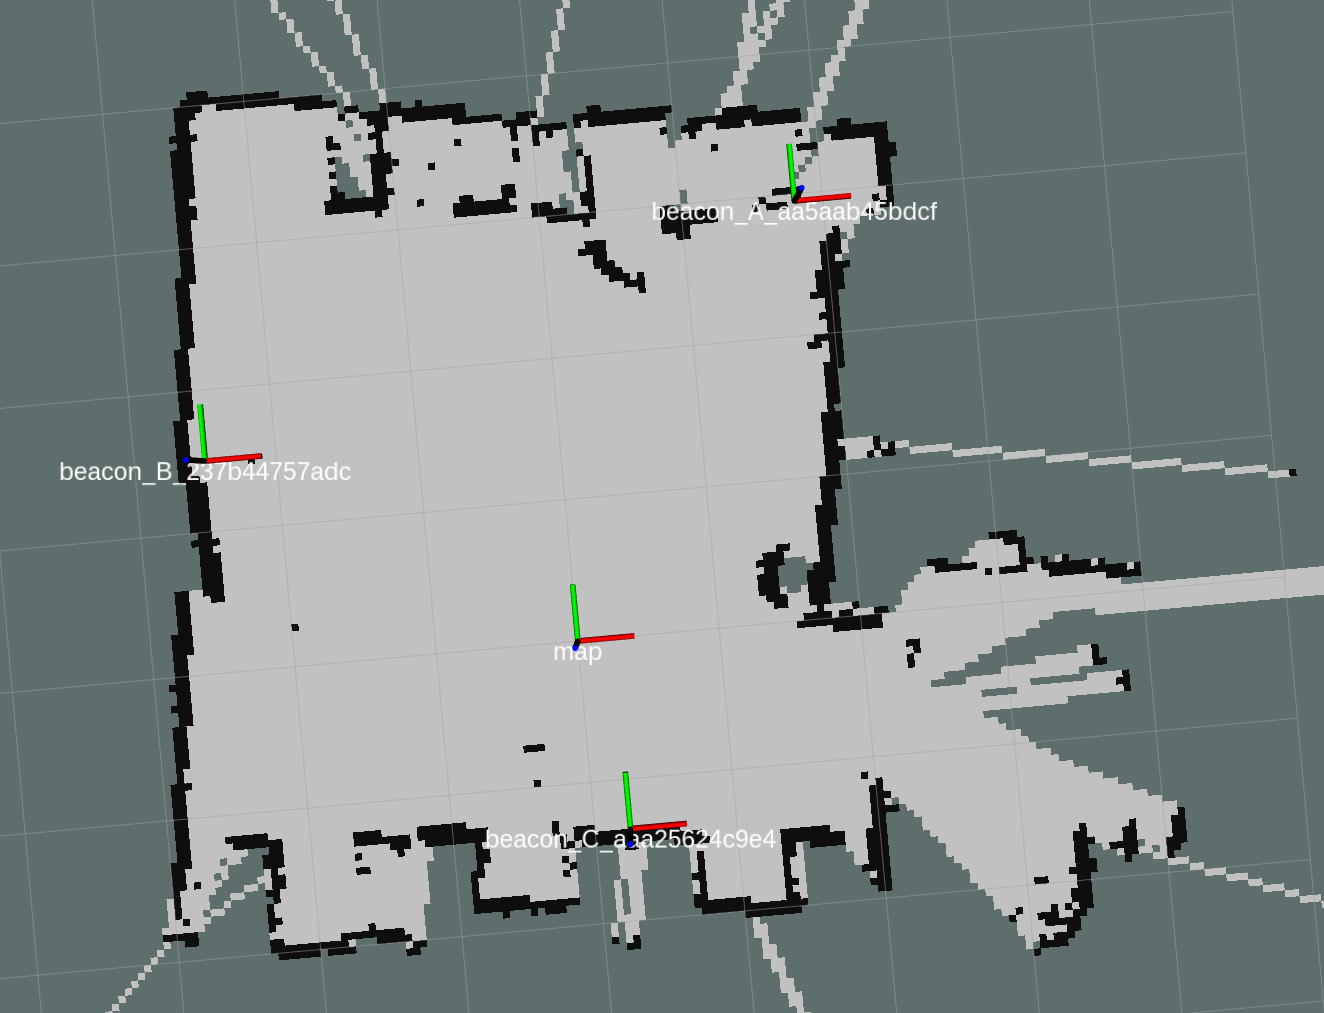
\includegraphics[width=0.9\textwidth]{img/mapa2.png}
\caption{Mapa środowiska wyznaczona metodą SLAM za pomocą programu GMapping z zaznaczonymi znacznikami radiowymi.}
\label{fig:mapa}
\end{figure}


\subsubsection{Kalibracja znaczników}

Tabela \ref{tab:strojenie} przedstawia wyniki kalibracji znaczników. Z wyników pomiaru usunięto punkty znacząco odbiegające od oczekiwanego przebiegu. Dopasowane krzywe wraz z punktami pomiarowymi wykreślono na rys. \ref{fig:strojenie-a}, \ref{fig:strojenie-b} oraz \ref{fig:strojenie-c}.

\begin{table}[H]
 \caption{Wyniki kalibracji}
 \label{tab:strojenie}
 \begin{tabular}{|l|l|l|}
  \hline
  \textbf{Znacznik}	& \textbf{Interpolacja} & \textbf{Dopasowanie krzywej potęgowej }\\ \hline
  A 		& $a=50,515$, $b=28,631$	& $a=50,167$, $b=28,480$	\\ \hline
  B 		& $a=65,036$, $b=11,547$	& $a=66,028$, $b=10,074$	\\ \hline
  C 		& $a=65,468$, $b=7,319$		& $a=68,215$, $b=0,984$		\\ \hline
 \end{tabular}

\end{table}


\begin{figure}[H]
\centering
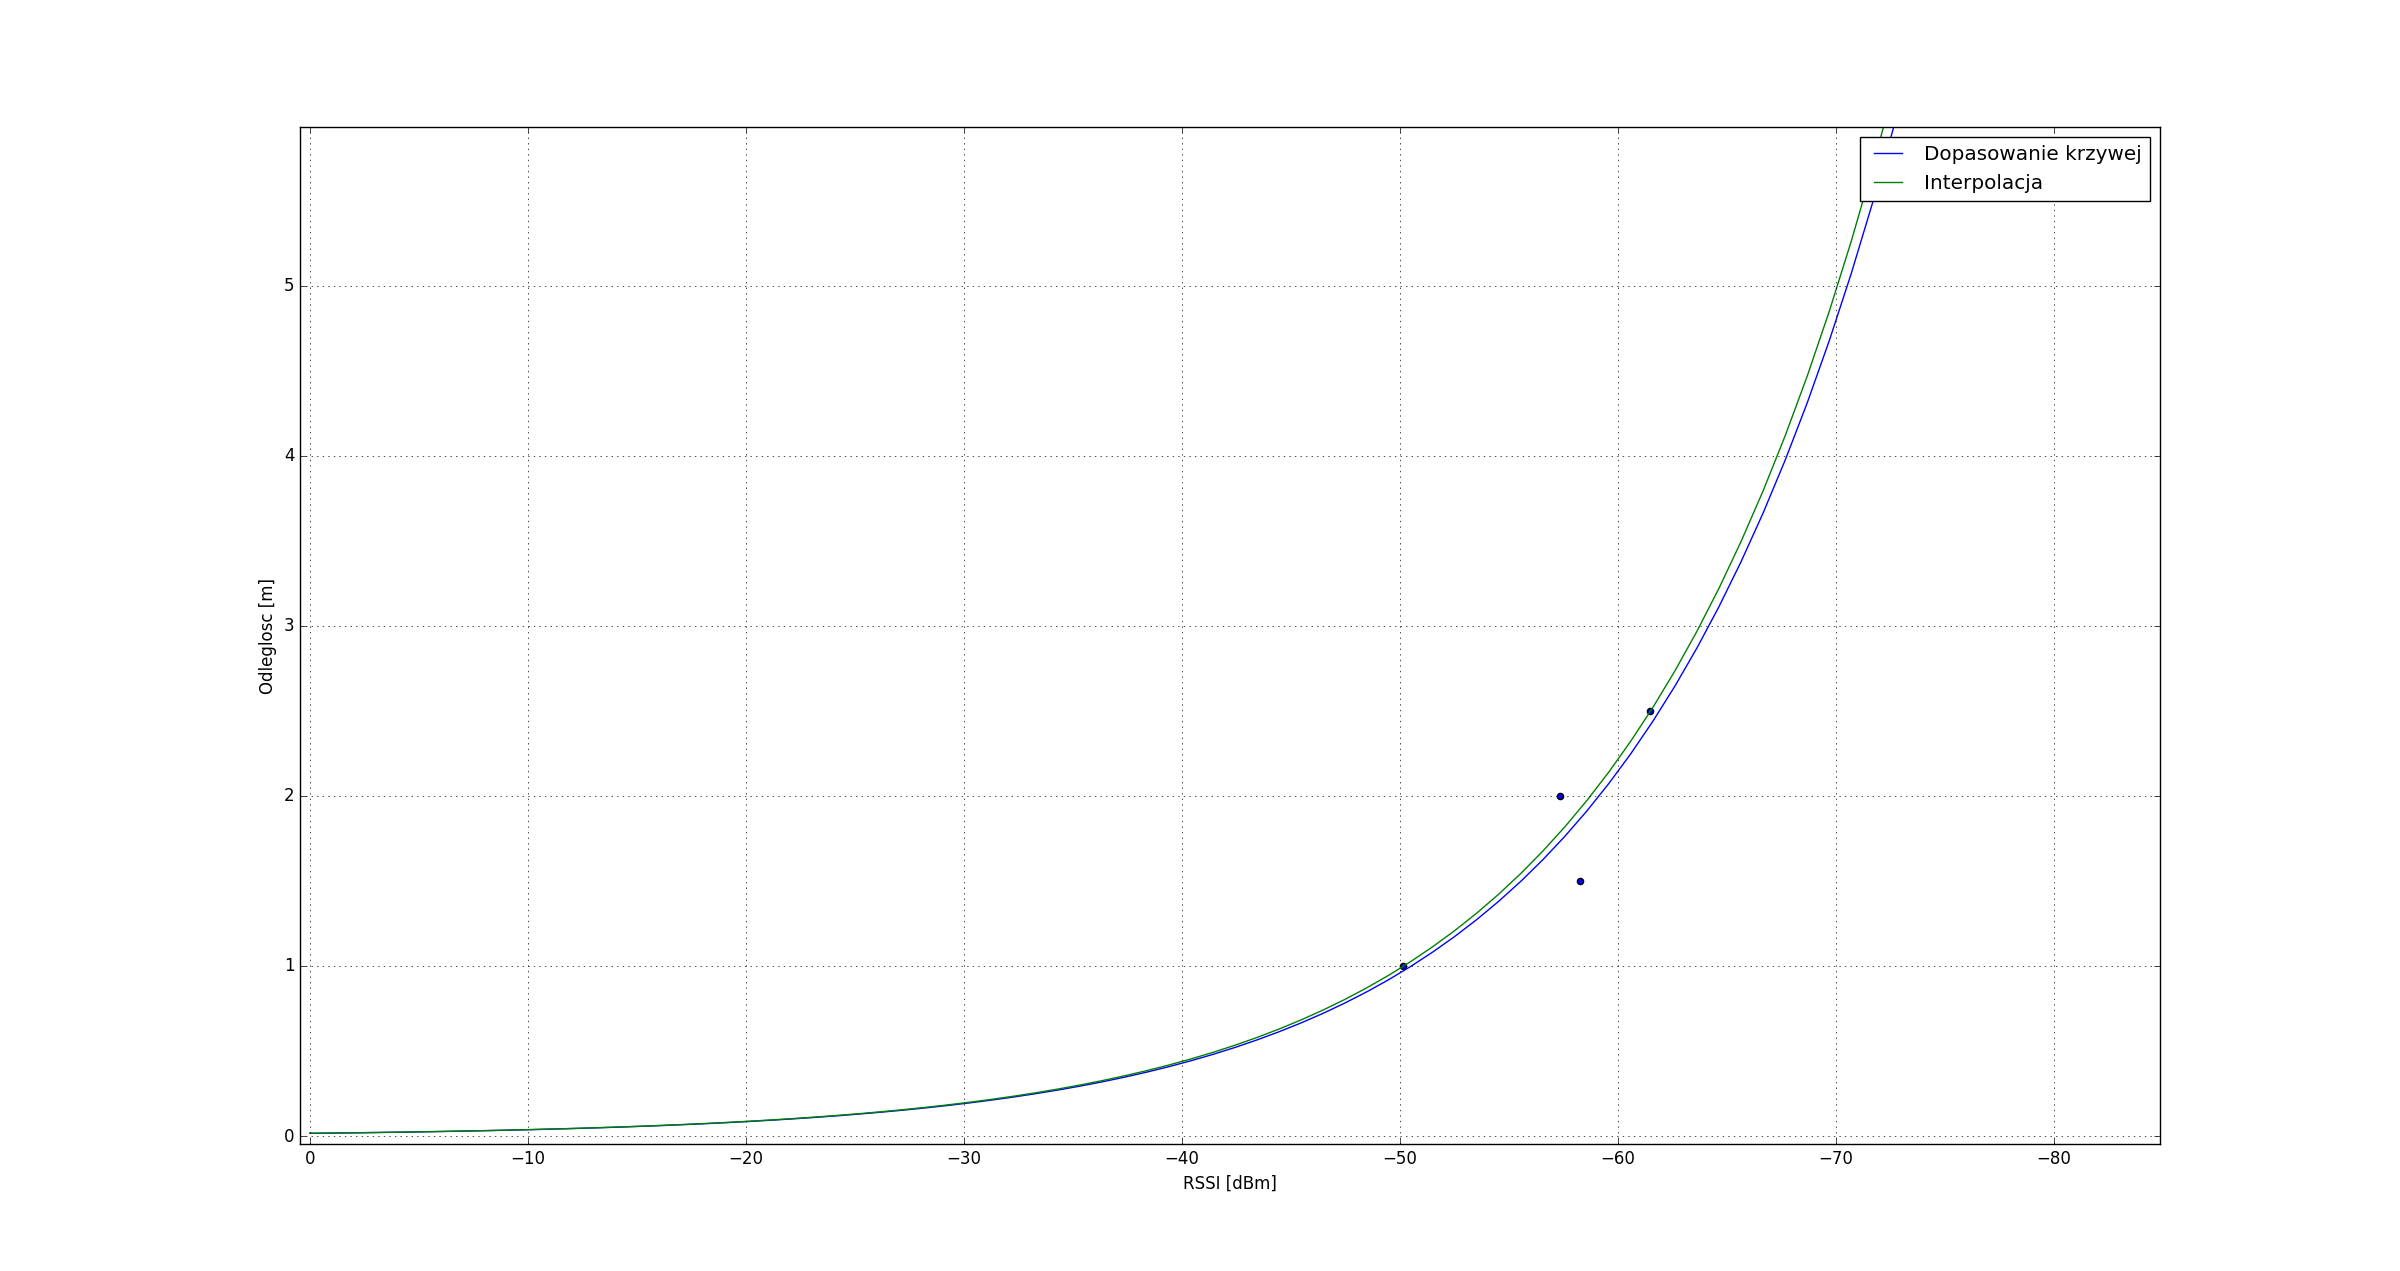
\includegraphics[width=1\textwidth]{img/strojenie-a.png}
\caption{Wyznaczanie modelu znacznika A}
\label{fig:strojenie-a}
\end{figure}

\begin{figure}[H]
\centering
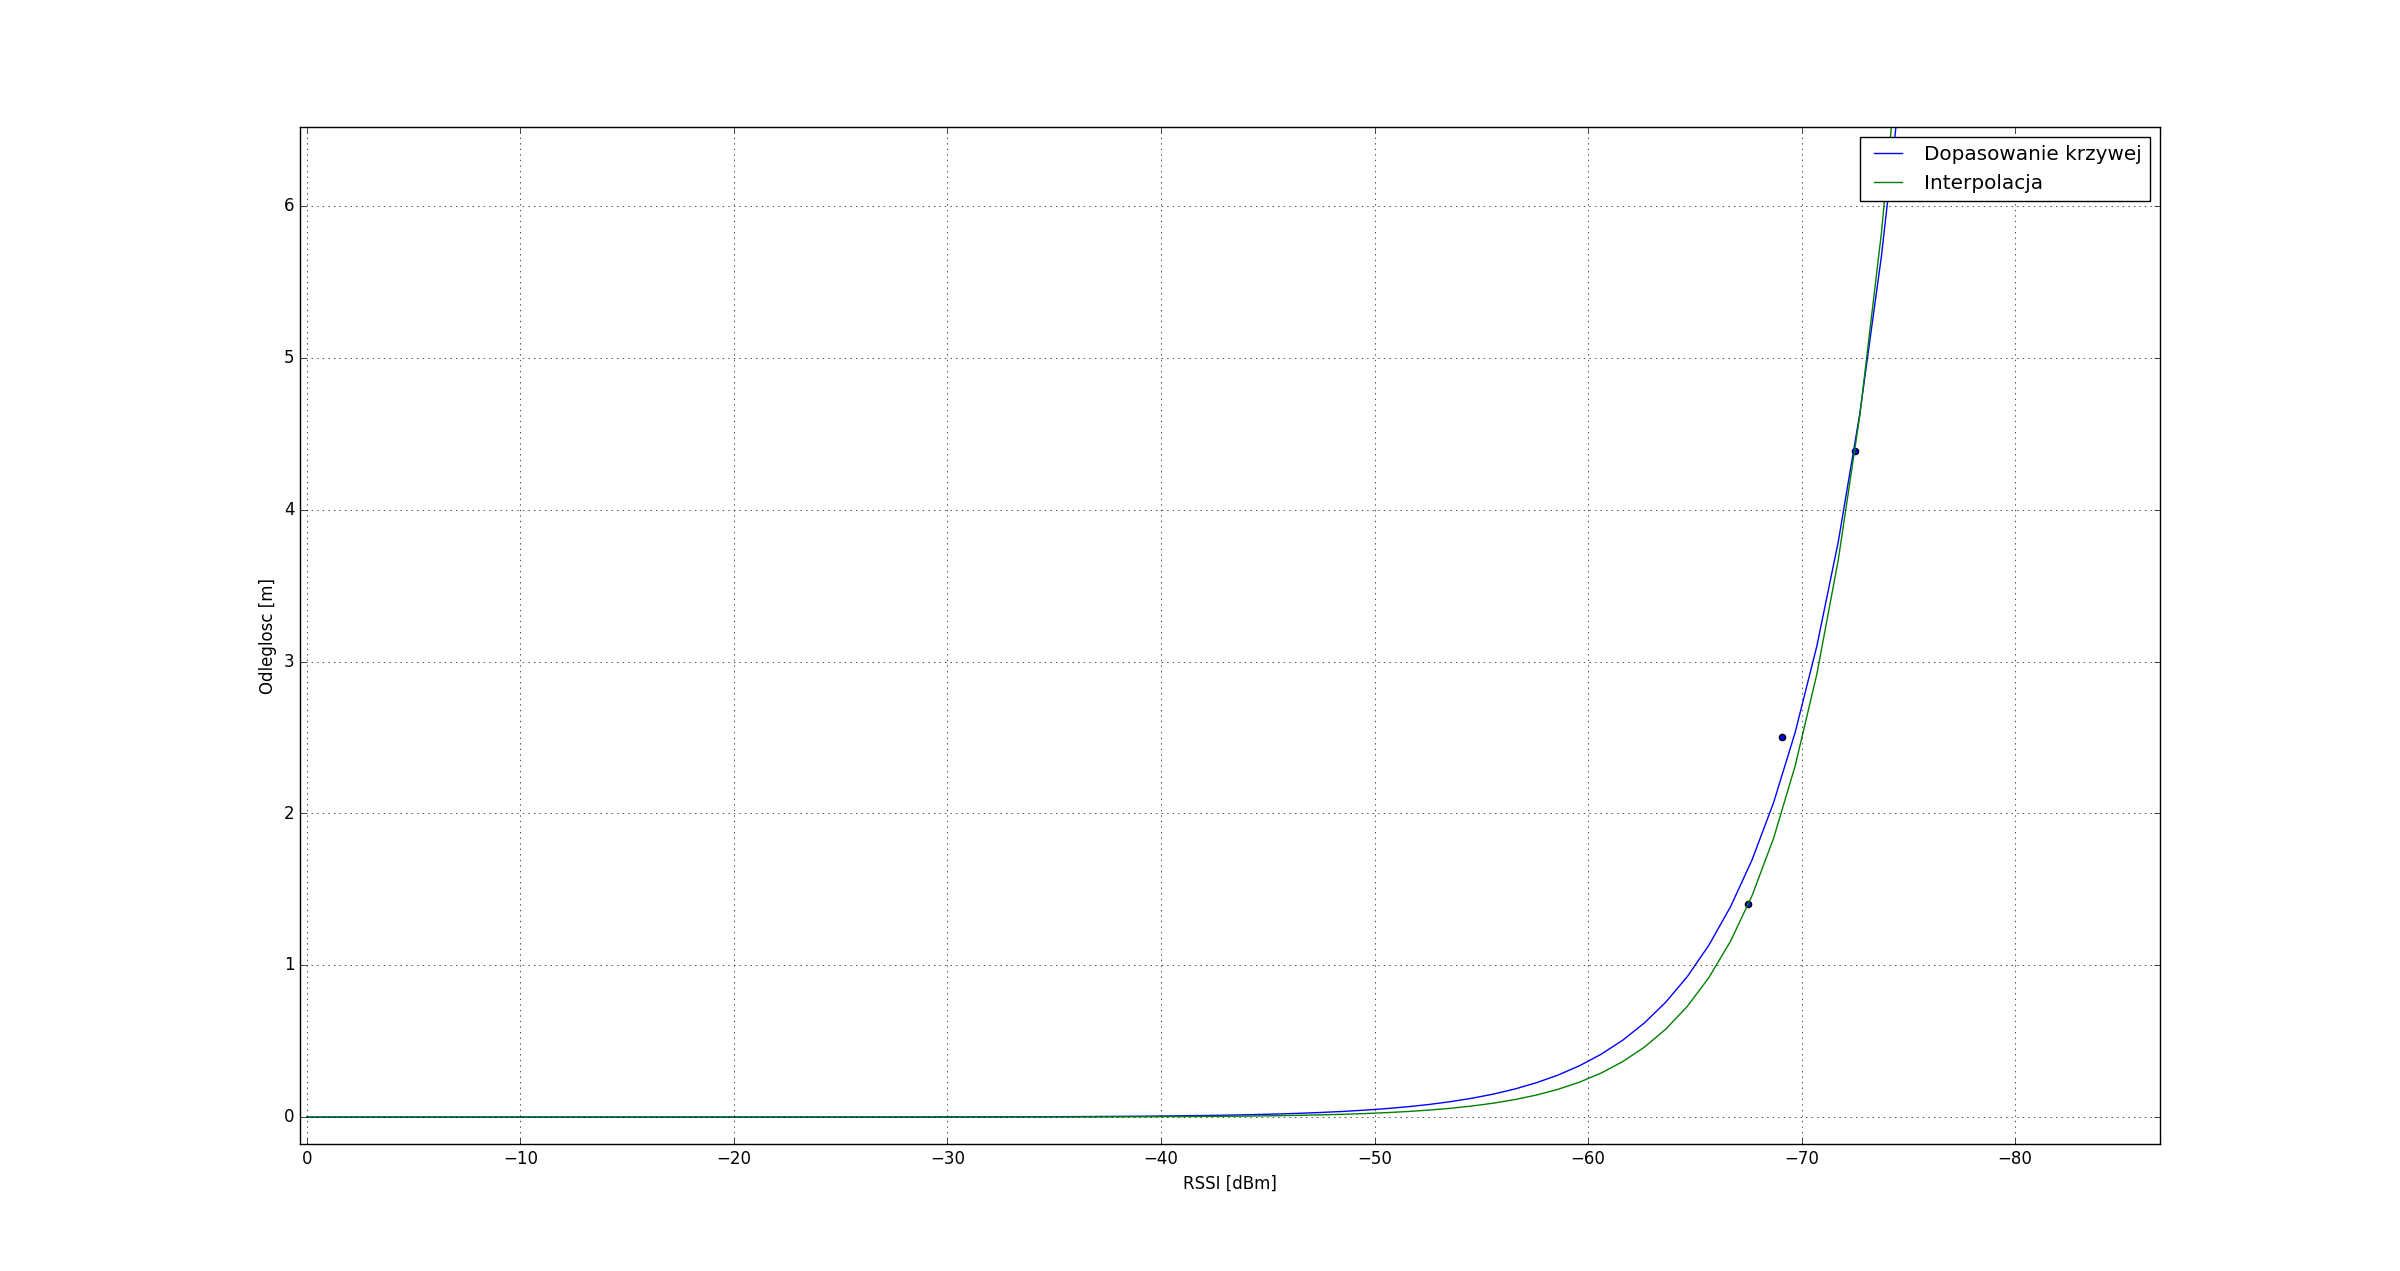
\includegraphics[width=1\textwidth]{img/strojenie-b.png}
\caption{Wyznaczanie modelu znacznika B}
\label{fig:strojenie-b}
\end{figure}

\begin{figure}[H]
\centering
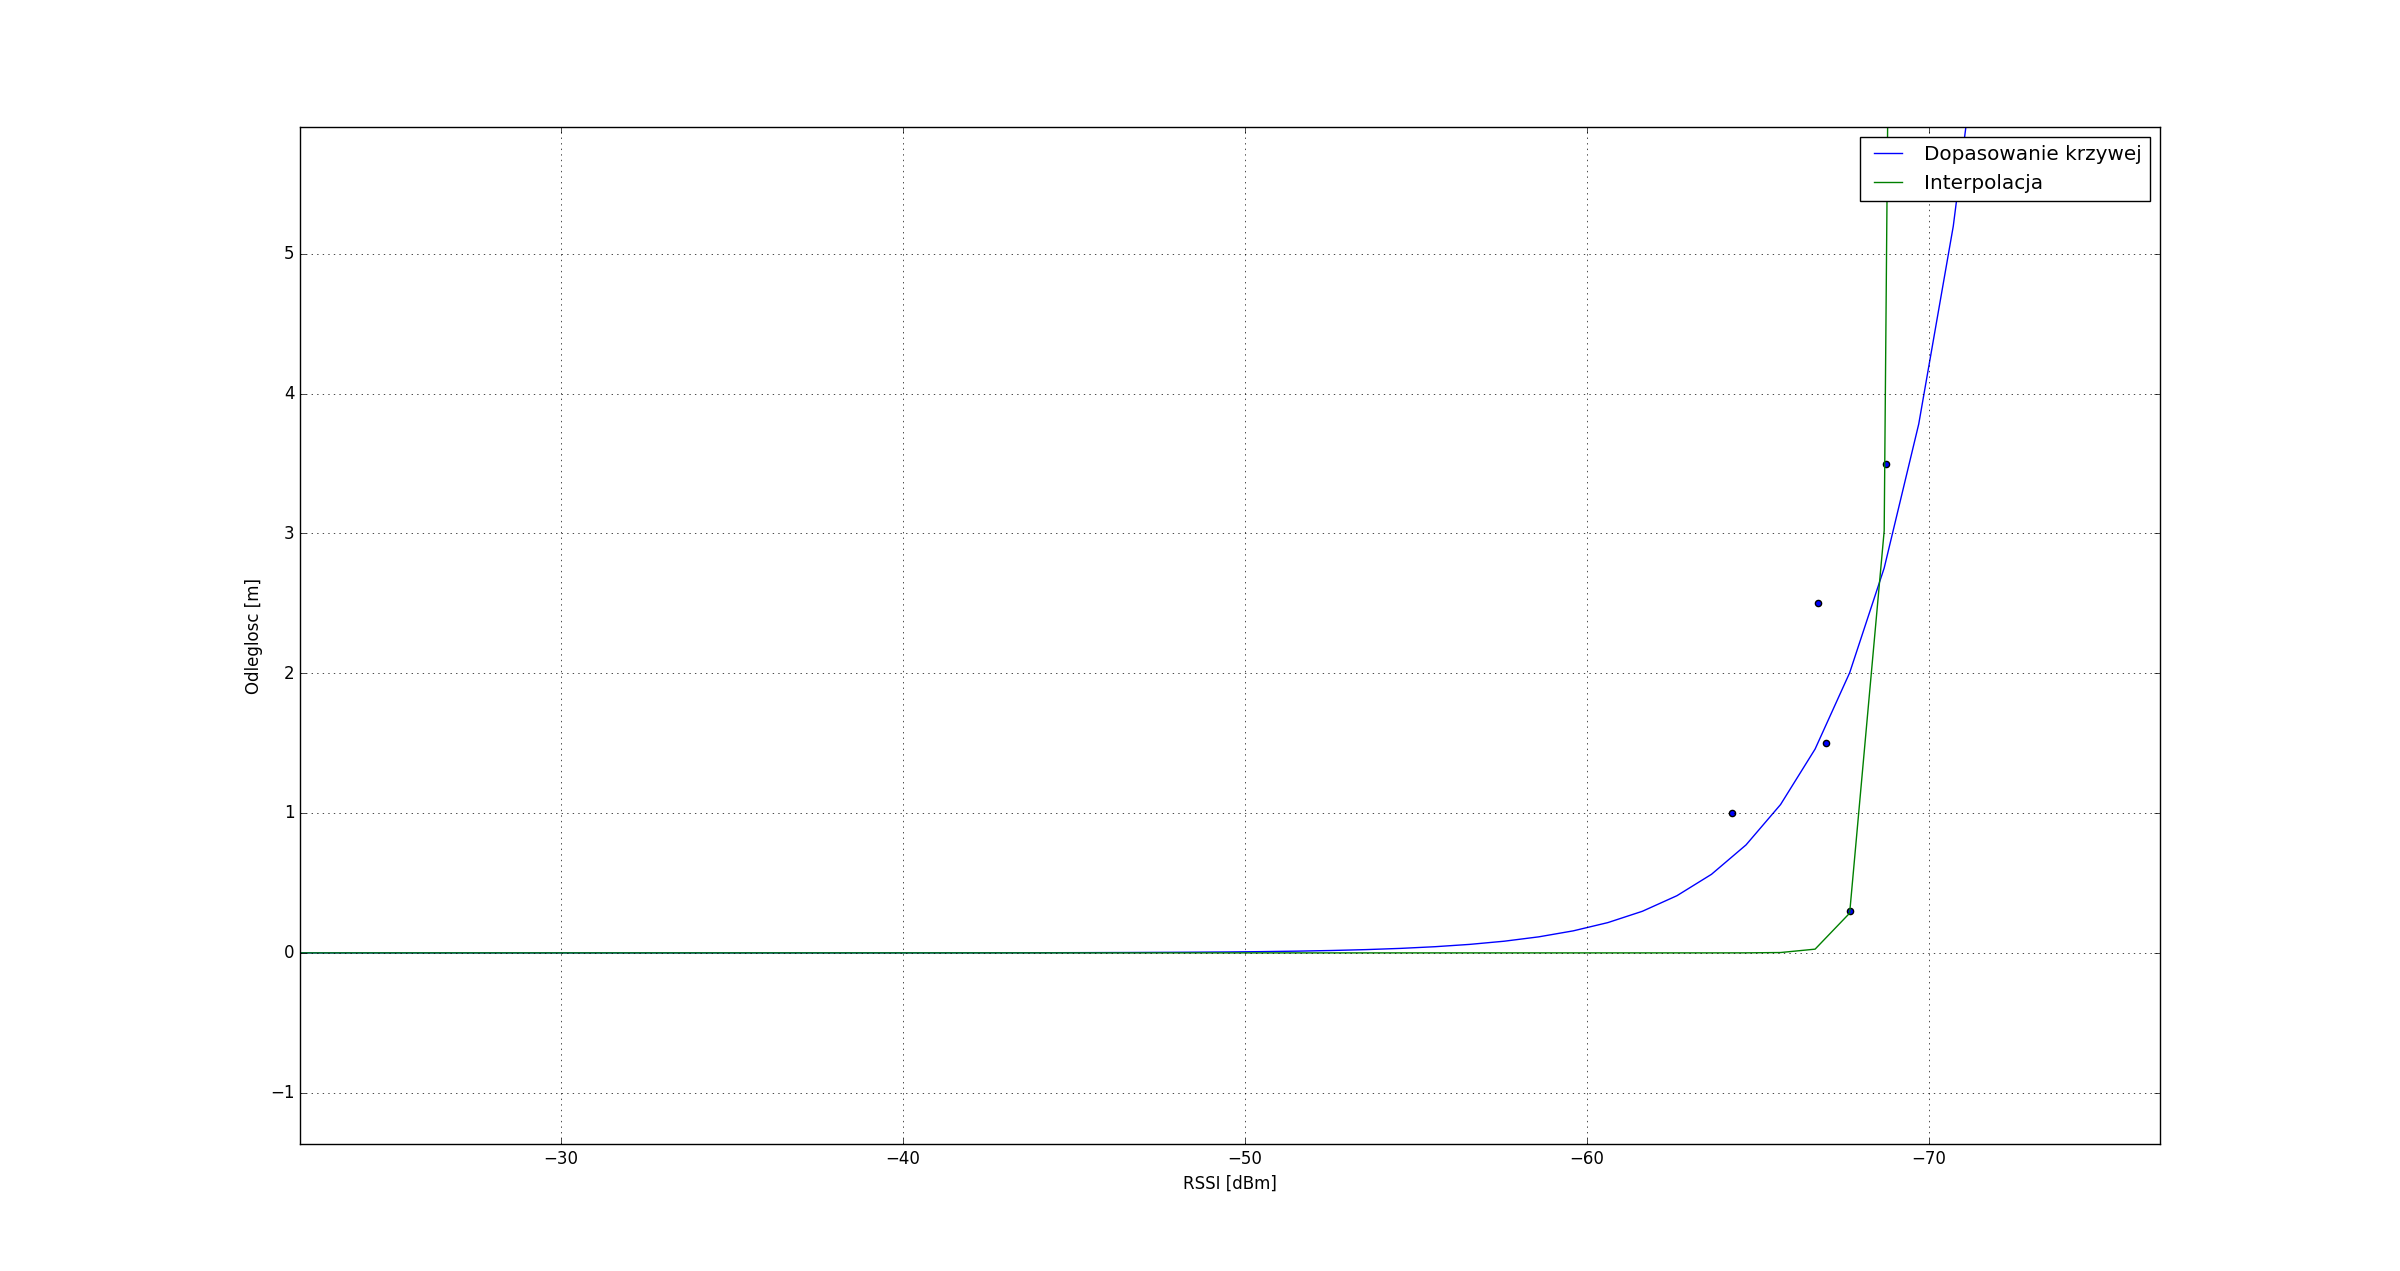
\includegraphics[width=1\textwidth]{img/strojenie-c.png}
\caption{Wyznaczanie modelu znacznika C}
\label{fig:strojenie-c}
\end{figure}

\subsubsection{Trilateracja}
Pierwsze próby lokalizacji za pomocą trilateracji przeprowadzono wykorzystując model wyznaczony w poprzednim punkcie metodą dopasowania krzywej. Jednakże, jak pokazuje rys. \ref{fig:trilat-przegryw}, nastawy te powodują bardzo duży rozrzut wyników pomiaru - większość wyznaczonych położeń robota wypada poza mapą i nie ma związku z rzeczywistym jego położeniem. Rys. \ref{fig:trilat-przegryw} obrazuje ten problem dla jednego punktu pomiarowego, jednakże podobnie duży rozrzut występuje również dla pozostałych punktów. Należy zwrócić uwagę na inną skalę osi wykresu \ref{fig:trilat-przegryw} w porównaniu do wykresów  \ref{fig:trilat-first} - \ref{fig:trilat-last}. Dyskusję możliwych przyczyn takiego zachowania przedstawiono w rozdziale \ref{ch:wnioski}.

Dlatego też podjęto próbę wyznaczenia właściwego modelu ręcznie, metodą prób i błędów. Bazując na modelach wyznacznonych automatycznie, wykorzystując narzędzie Rosbag oraz narzędzia do wykreślania zależności siły sygnału od odległości, dobrano model zapewniający wyniki o mniejszym rozrzucie:
\begin{equation}
 a=50, b=50
\end{equation}

Wyniki z wykorzystaniem modelu wyznaczonego ręcznie pokazują rys. \ref{fig:trilat-first} - \ref{fig:trilat-last}. Dla porównania, rysunki te, z wyjątkiem rys. \ref{fig:trilat-przegryw} posiadają jednakową skalę. Rysunek \ref{fig:trilat-przegryw} ma zmienioną skalę aby ukazać problem rozrzutu wyników. 

Na rysunkach, czerwony krzyżyk oznacza punkt odniesienia, niebieskie kropki symbolizują wyniki trilateracji. Na rysunku \ref{fig:referencyjne} przedstawiono położenie kolejnych punktów odniesienia.
\begin{figure}[H]
\centering
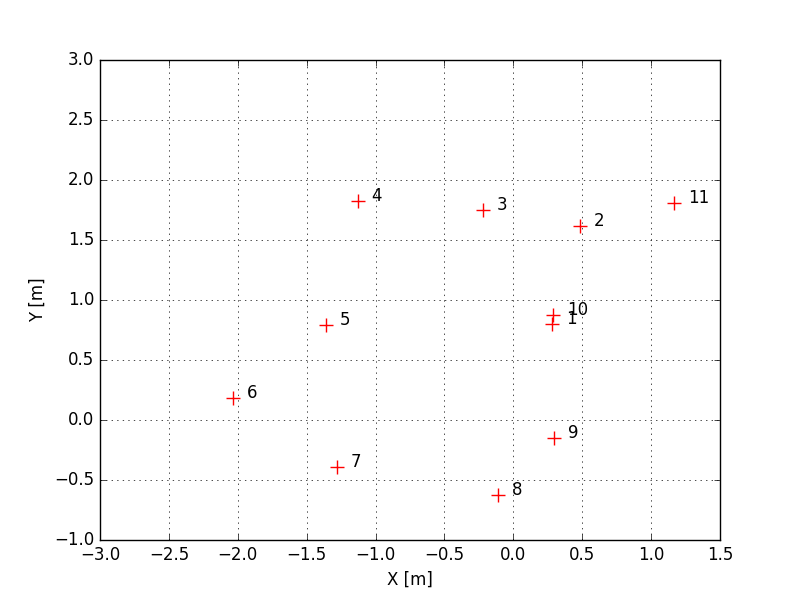
\includegraphics[width=0.7\textwidth]{img/references.png}
\caption{Położenie punktów pomiarowych.}
\label{fig:referencyjne}
\end{figure}
\begin{figure}[H]
\centering
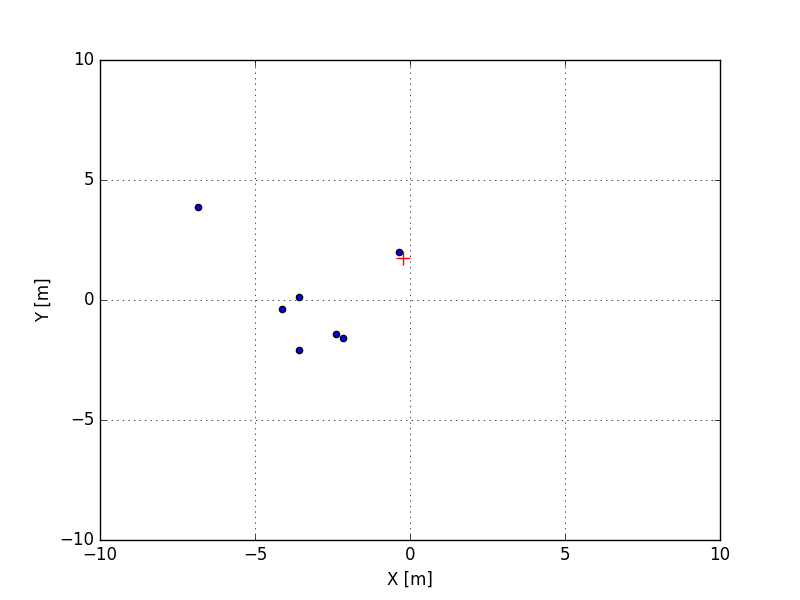
\includegraphics[width=0.7\textwidth]{img/trilat-przegryw.png}
\caption{Wyniki trilateracji dla modelu obliczonego przez dopasowanie krzywej}
\label{fig:trilat-przegryw}
\end{figure}
\begin{figure}[H]
\centering
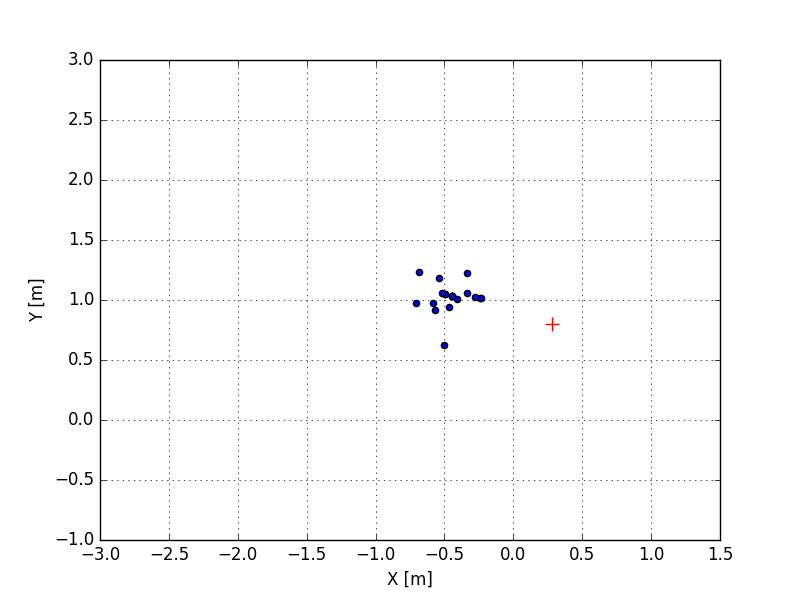
\includegraphics[width=0.7\textwidth]{img/trilat-map3-1.png}
\caption{Wyniki trilateracji dla ręcznie dobranego modelu - punkt 1}
\label{fig:trilat-first}
\end{figure}
\begin{figure}[H]
\centering
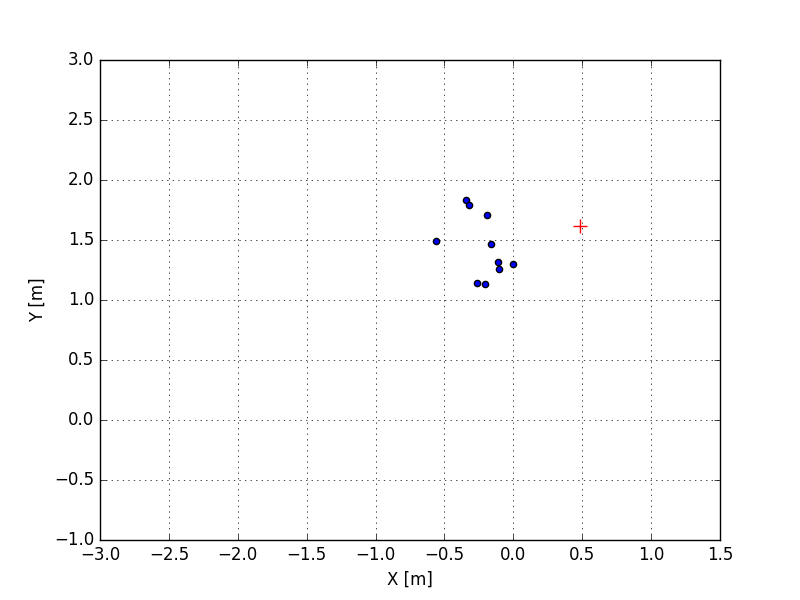
\includegraphics[width=0.7\textwidth]{img/trilat-map3-2.png}
\caption{Wyniki trilateracji dla ręcznie dobranego modelu - punkt 2}
\end{figure}
\begin{figure}[H]
\centering
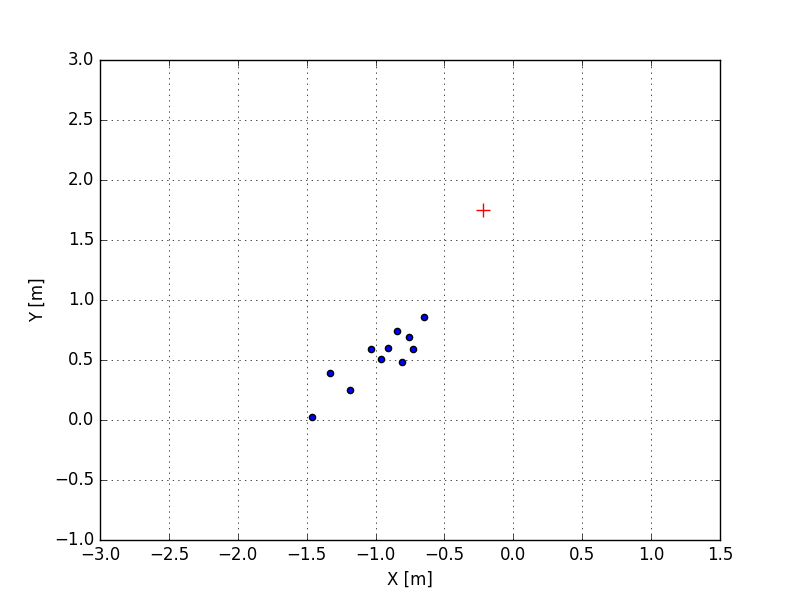
\includegraphics[width=0.7\textwidth]{img/trilat-map3-3.png}
\caption{Wyniki trilateracji dla ręcznie dobranego modelu - punkt 3}
\end{figure}
\begin{figure}[H]
\centering
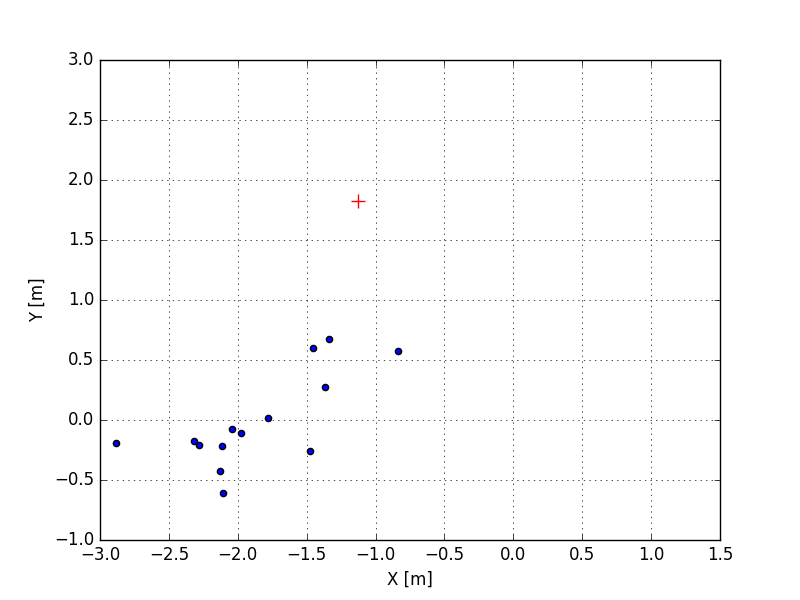
\includegraphics[width=0.7\textwidth]{img/trilat-map3-4.png}
\caption{Wyniki trilateracji dla ręcznie dobranego modelu - punkt 4}
\end{figure}
\begin{figure}[H]
\centering
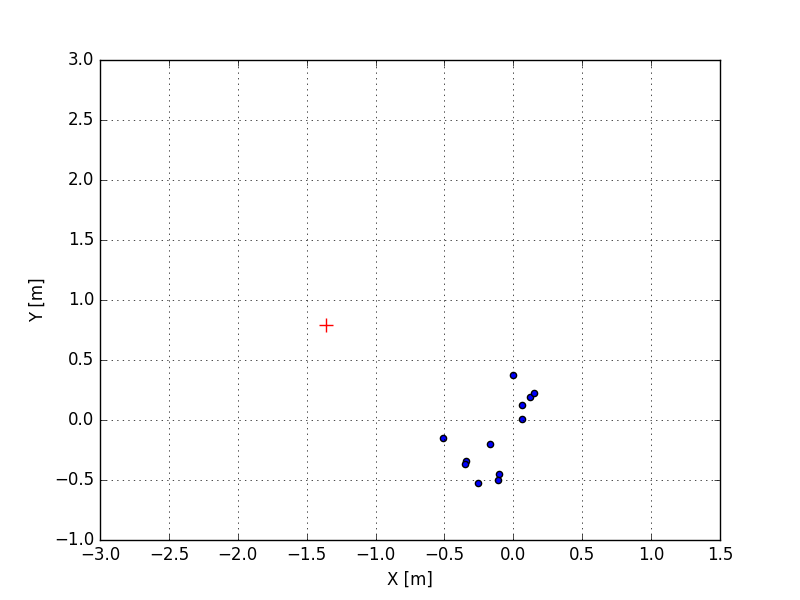
\includegraphics[width=0.7\textwidth]{img/trilat-map3-5.png}
\caption{Wyniki trilateracji dla ręcznie dobranego modelu - punkt 5}
\end{figure}
\begin{figure}[H]
\centering
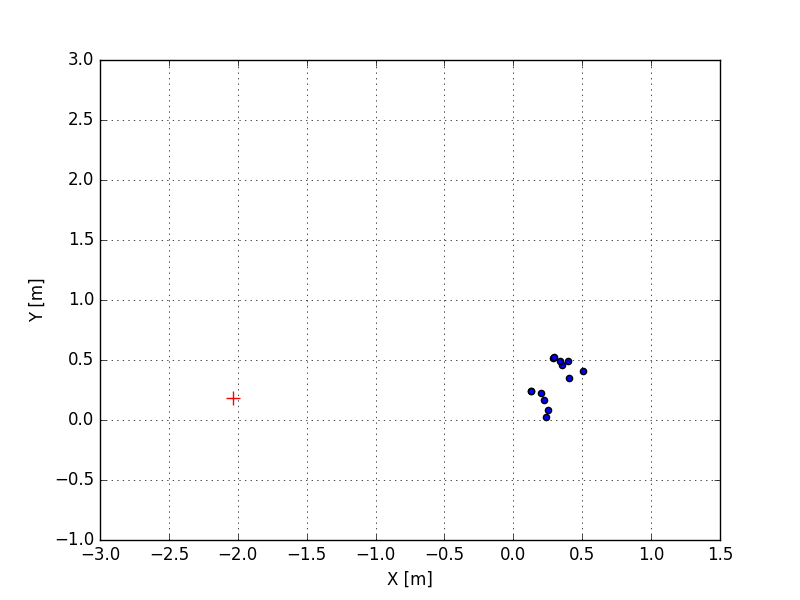
\includegraphics[width=0.7\textwidth]{img/trilat-map3-6.png}
\caption{Wyniki trilateracji dla ręcznie dobranego modelu - punkt 6}
\end{figure}
\begin{figure}[H]
\centering
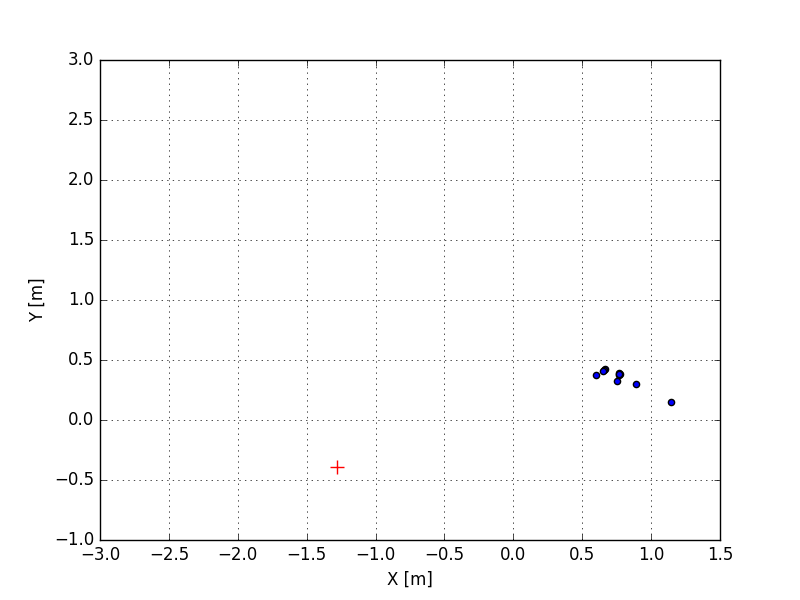
\includegraphics[width=0.7\textwidth]{img/trilat-map3-7.png}
\caption{Wyniki trilateracji dla ręcznie dobranego modelu - punkt 7}
\end{figure}
\begin{figure}[H]
\centering
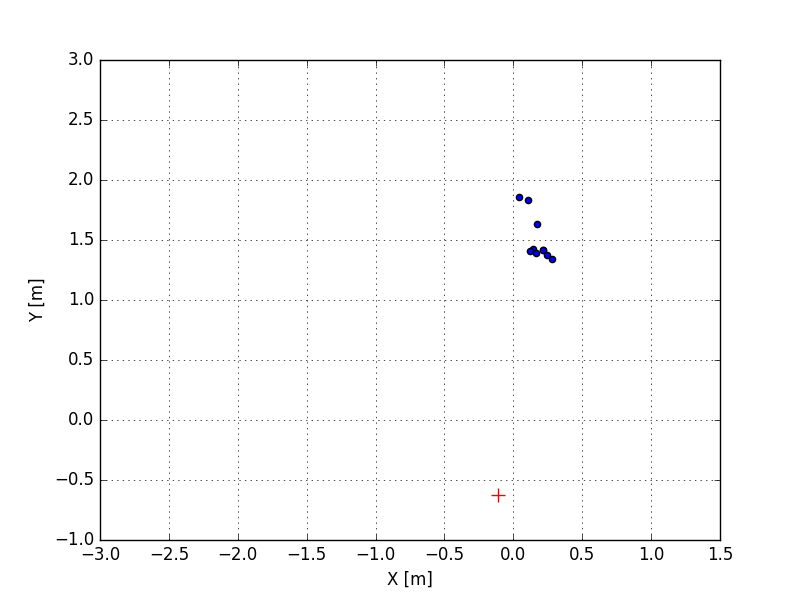
\includegraphics[width=0.7\textwidth]{img/trilat-map3-8.png}
\caption{Wyniki trilateracji dla ręcznie dobranego modelu - punkt 8}
\end{figure}
\begin{figure}[H]
\centering
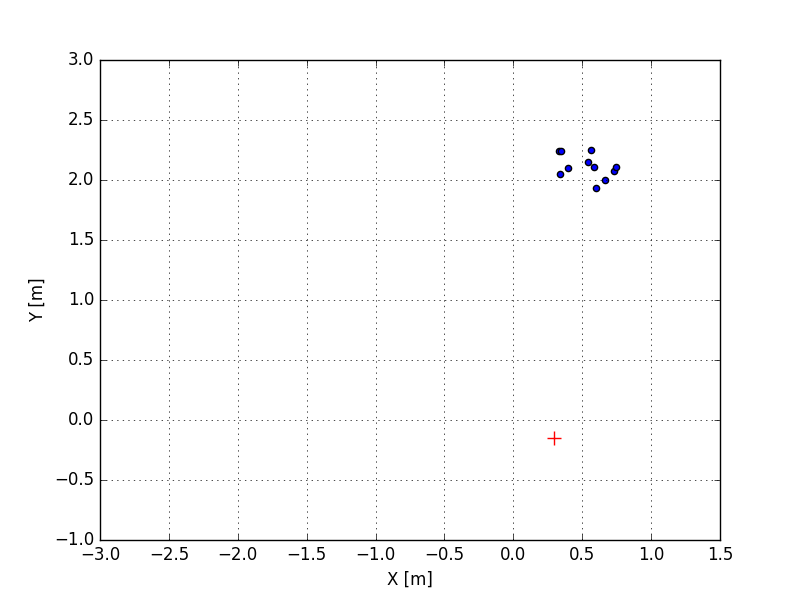
\includegraphics[width=0.7\textwidth]{img/trilat-map3-9.png}
\caption{Wyniki trilateracji dla ręcznie dobranego modelu - punkt 9}
\end{figure}
\begin{figure}[H]
\centering
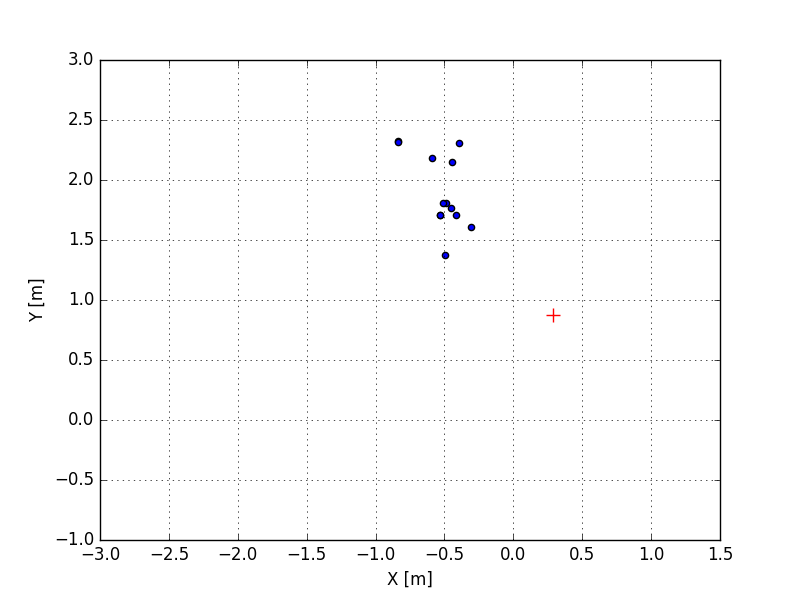
\includegraphics[width=0.7\textwidth]{img/trilat-map3-10.png}
\caption{Wyniki trilateracji dla ręcznie dobranego modelu - punkt 10}
\end{figure}
\begin{figure}[H]
\centering
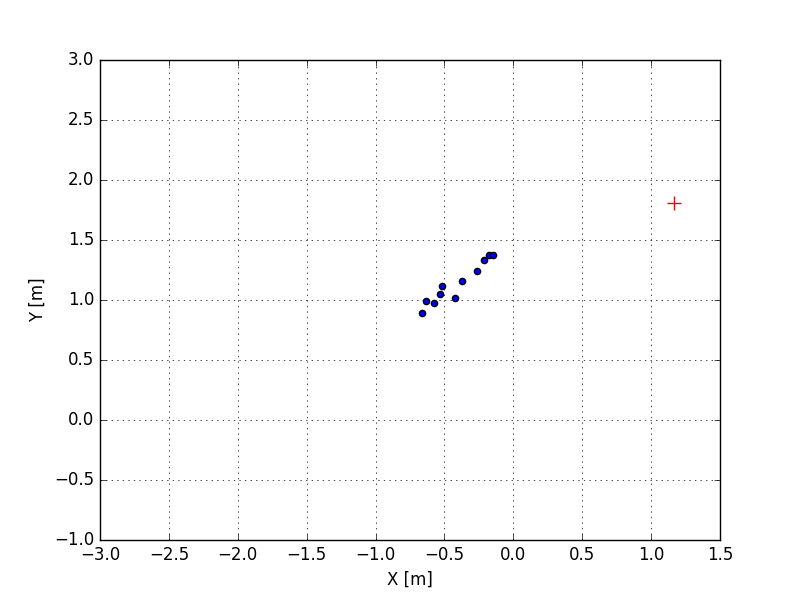
\includegraphics[width=0.7\textwidth]{img/trilat-map3-11.png}
\caption{Wyniki trilateracji dla ręcznie dobranego modelu - punkt 11}
\label{fig:trilat-last}
\end{figure}


\subsubsection{Filtr cząsteczkowy}
Jak wspomniano wcześniej, badanie filtra cząsteczkowego przeprowadzono na tym samym zbiorze danych co badania metody trilateracji. Podobnie jak w wypadku trilateracji, wykorzystano model wyznacznony ręcznie. Wyniki lokalizacji w poszczególnych punktach ukazują wykresy \ref{fig:pf-first} - \ref{fig:pf-last}. Można zauważyć, że na wykresach zaznaczono miejszą ilość punktów wynikowych niż w wypadku trilateracji. Ta różnica wynika z faktu, że wynik trilateracji jest publikowany w stałym interwale (1 sekunda), natomiast filtr cząsteczkowy jest przeliczany tylko wtedy, kiedy odległość liniowa lub kątowa pokonana przez robota i zmierzona za pomocą odometrii przekroczy pewien próg. Jest to związane z optymalizacją wydajności programu. Dlatego też, kiedy robot jest nieruchomy, nowe punkty nie są publikowane - bowiem byłyby identyczne jak poprzednie.


\begin{figure}[H]
\centering
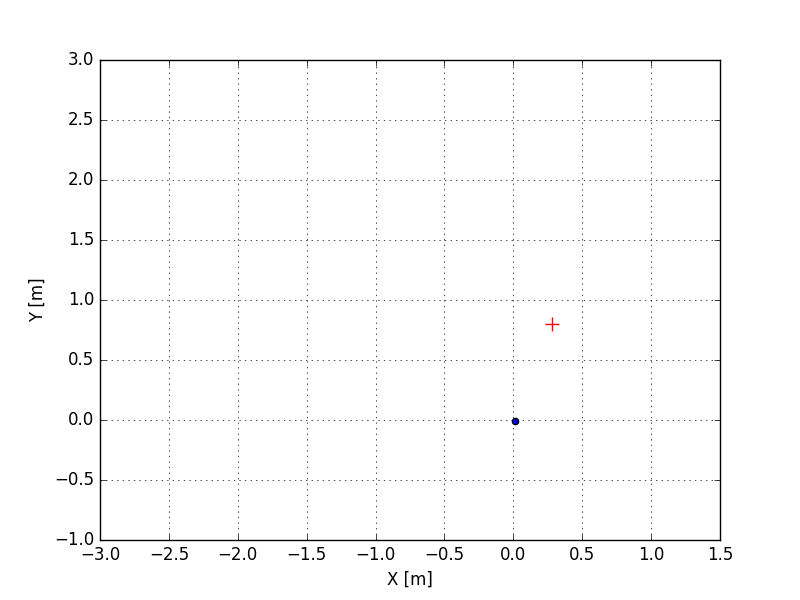
\includegraphics[width=0.7\textwidth]{img/pf-map3-1.png}
\caption{Wyniki lokalizacji za pomocą filtra cząsteczkowego dla ręcznie dobranego modelu - punkt 1}
\label{fig:pf-first}
\end{figure}
\begin{figure}[H]
\centering
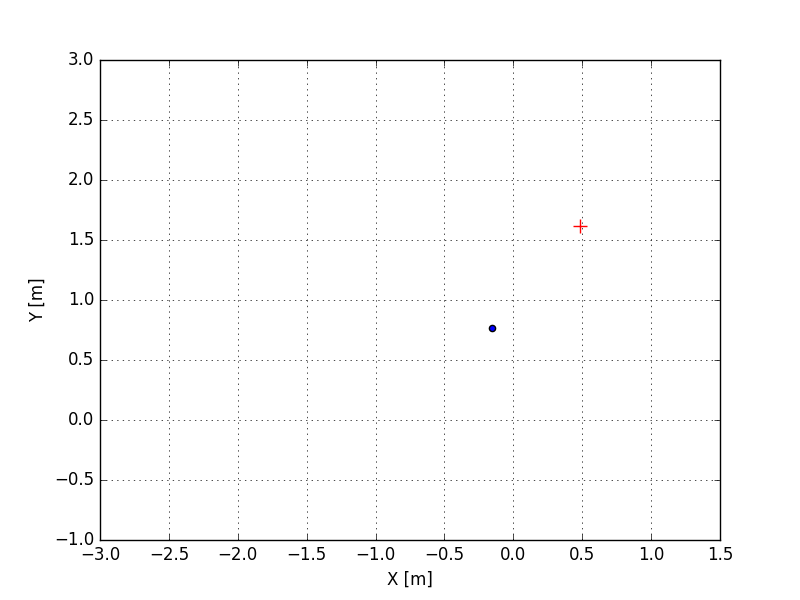
\includegraphics[width=0.7\textwidth]{img/pf-map3-2.png}
\caption{Wyniki lokalizacji za pomocą filtra cząsteczkowego dla ręcznie dobranego modelu - punkt 2}
\end{figure}
\begin{figure}[H]
\centering
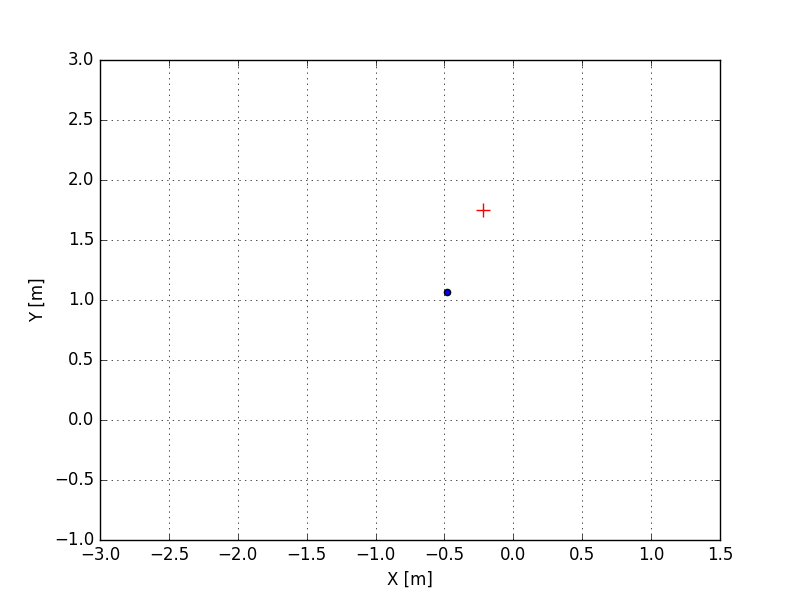
\includegraphics[width=0.7\textwidth]{img/pf-map3-3.png}
\caption{Wyniki lokalizacji za pomocą filtra cząsteczkowego dla ręcznie dobranego modelu - punkt 3}
\end{figure}
\begin{figure}[H]
\centering
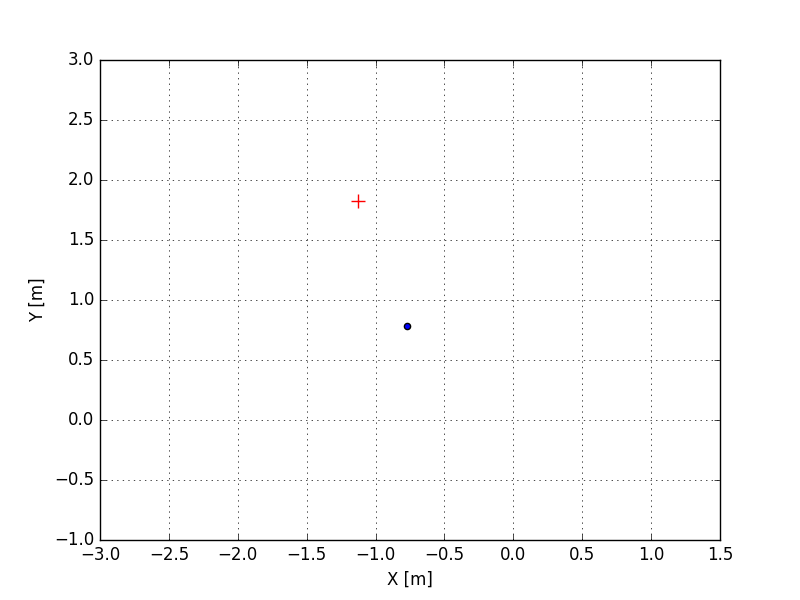
\includegraphics[width=0.7\textwidth]{img/pf-map3-4.png}
\caption{Wyniki lokalizacji za pomocą filtra cząsteczkowego dla ręcznie dobranego modelu - punkt 4}
\end{figure}
\begin{figure}[H]
\centering
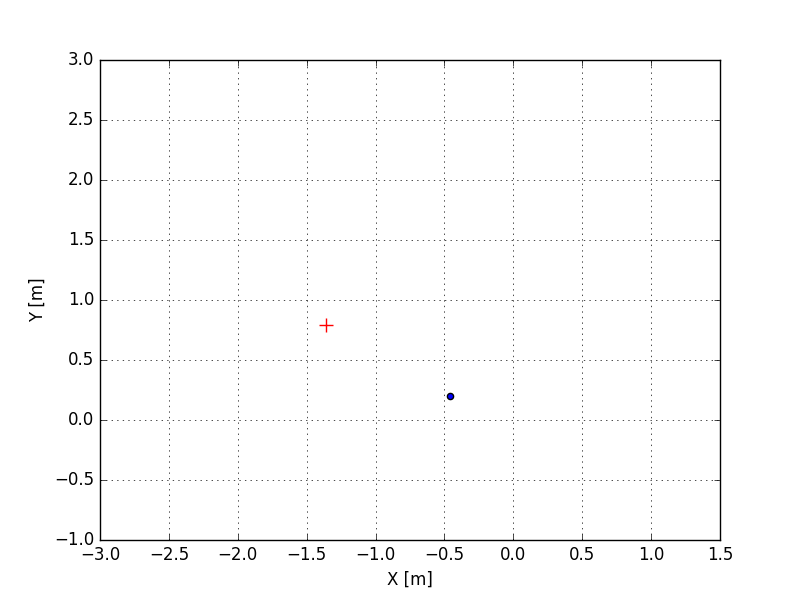
\includegraphics[width=0.7\textwidth]{img/pf-map3-5.png}
\caption{Wyniki lokalizacji za pomocą filtra cząsteczkowego dla ręcznie dobranego modelu - punkt 5}
\end{figure}
\begin{figure}[H]
\centering
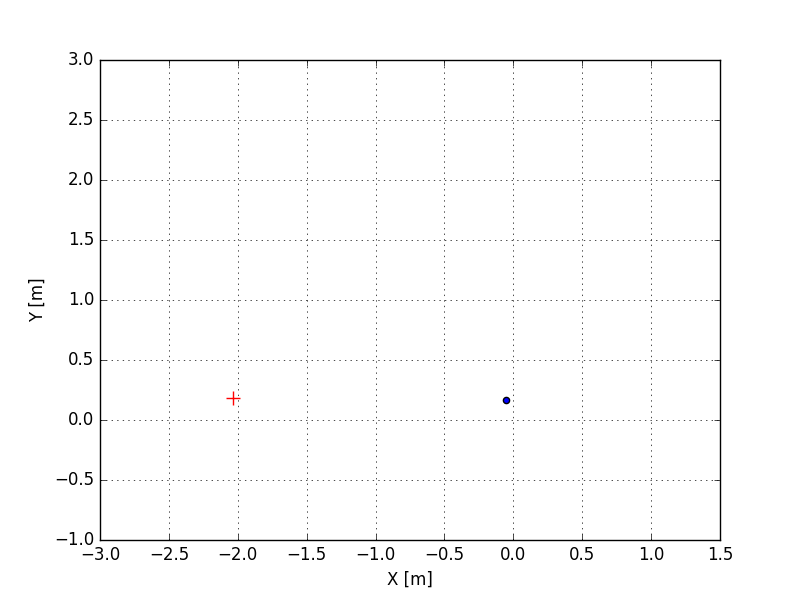
\includegraphics[width=0.7\textwidth]{img/pf-map3-6.png}
\caption{Wyniki lokalizacji za pomocą filtra cząsteczkowego dla ręcznie dobranego modelu - punkt 6}
\end{figure}
\begin{figure}[H]
\centering
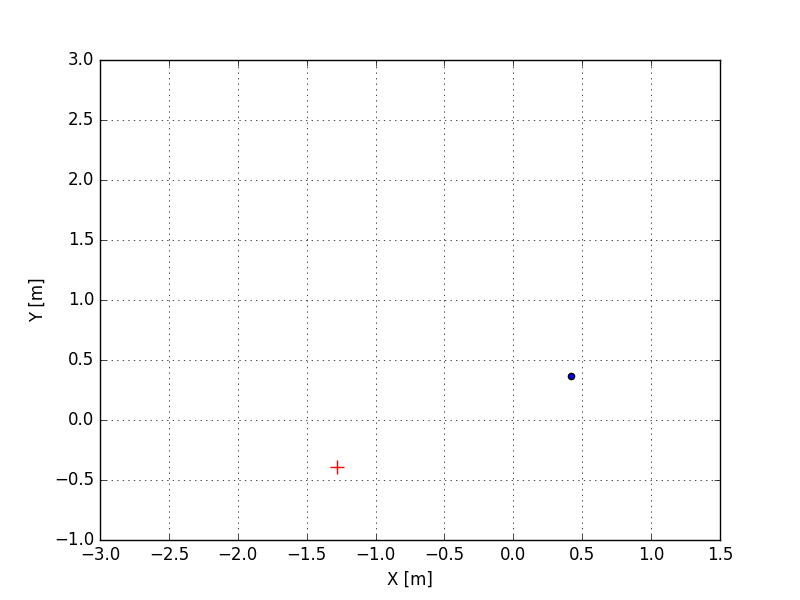
\includegraphics[width=0.7\textwidth]{img/pf-map3-7.png}
\caption{Wyniki lokalizacji za pomocą filtra cząsteczkowego dla ręcznie dobranego modelu - punkt 7}
\end{figure}
\begin{figure}[H]
\centering
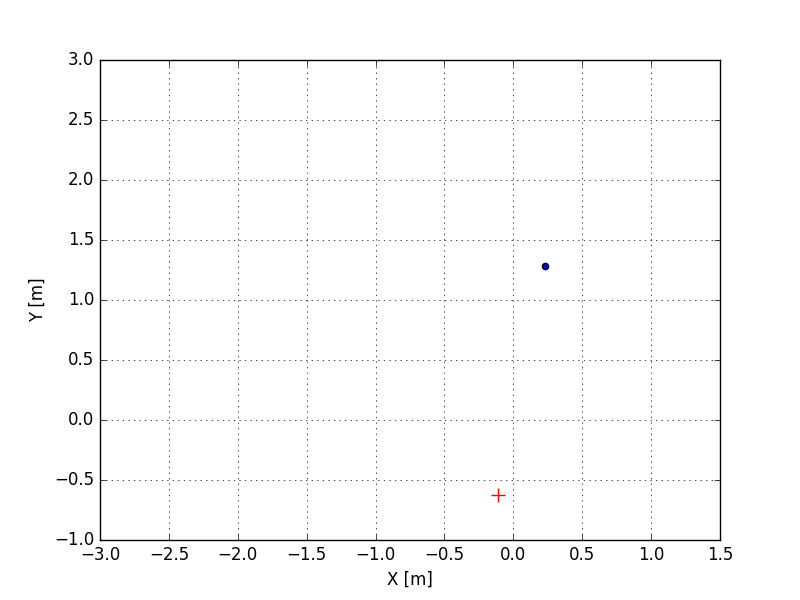
\includegraphics[width=0.7\textwidth]{img/pf-map3-8.png}
\caption{Wyniki lokalizacji za pomocą filtra cząsteczkowego dla ręcznie dobranego modelu - punkt 8}
\end{figure}
\begin{figure}[H]
\centering
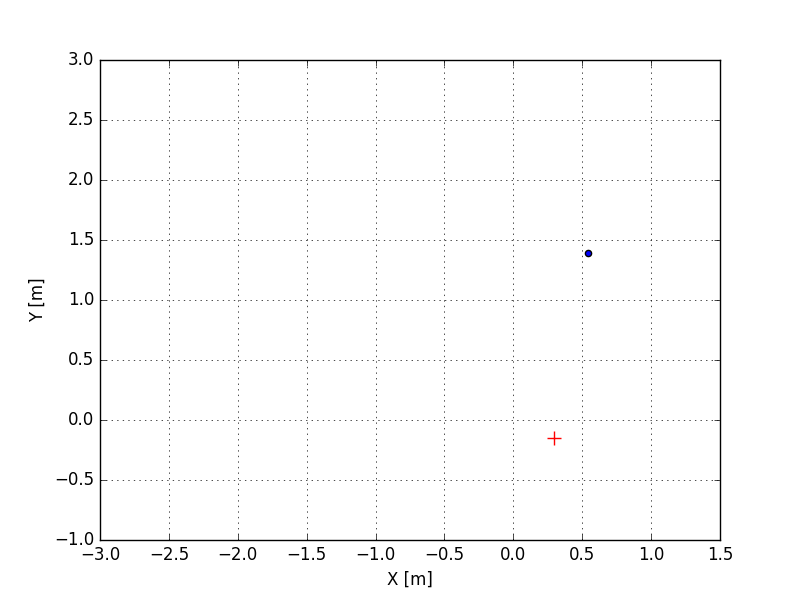
\includegraphics[width=0.7\textwidth]{img/pf-map3-9.png}
\caption{Wyniki lokalizacji za pomocą filtra cząsteczkowego dla ręcznie dobranego modelu - punkt 9}
\end{figure}
\begin{figure}[H]
\centering
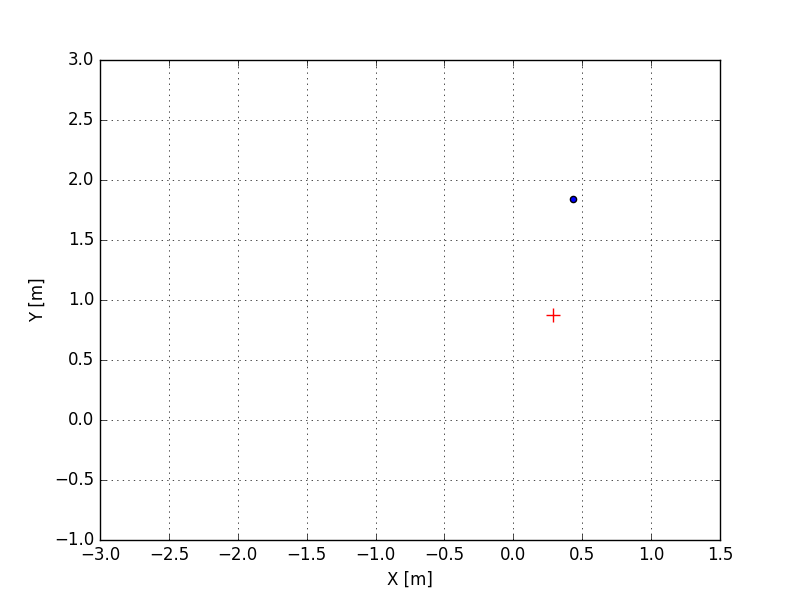
\includegraphics[width=0.7\textwidth]{img/pf-map3-10.png}
\caption{Wyniki lokalizacji za pomocą filtra cząsteczkowego dla ręcznie dobranego modelu - punkt 10}
\end{figure}
\begin{figure}[H]
\centering
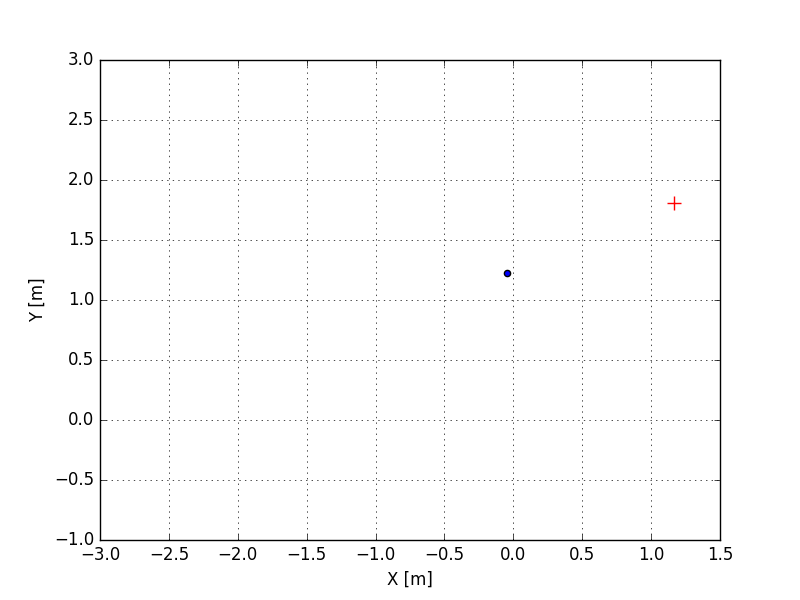
\includegraphics[width=0.7\textwidth]{img/pf-map3-11.png}
\caption{Wyniki lokalizacji za pomocą filtra cząsteczkowego dla ręcznie dobranego modelu - punkt 11}
\label{fig:pf-last}
\end{figure}

\section{Rozwiązanie problemu porwanego robota za pomocą lokalizacji BLE i AMCL}

